% --- Module 2 ---

\chapter{Principal Component Analysis (PCA)}

\section{Empirical Covariance Matrices}

Before deriving PCA, it is useful to make explicit the role of the \emph{empirical covariance matrix}:
it is the object PCA works on directly.

\textbf{Setting.} We have $n$ observations $x_1, \dots, x_n \in \mathbb{R}^p$, i.e.\ $n$ individuals
on which we measure $p$ variables. We write $x_{ij}$ for the $j$-th variable of the $i$-th observation.

\dfn{Empirical mean}{
  The \emph{empirical mean} of the dataset is the vector
  \[
    \bar{x} = \frac{1}{n}\sum_{i=1}^{n} x_i =
    \begin{bmatrix} \bar{x}_1 \\ \bar{x}_2 \\ \vdots \\ \bar{x}_p \end{bmatrix} \in \mathbb{R}^p,
    \qquad \bar{x}_j = \frac{1}{n}\sum_{i=1}^{n} x_{ij}.
  \]
  Each component $\bar{x}_j$ is simply the mean of the $j$-th variable.
}

\dfn{Empirical variance}{
  The \emph{empirical variance} of the $j$-th variable is
  \[
    s_j^2 = \frac{1}{n}\sum_{i=1}^{n} (x_{ij} - \bar{x}_j)^2 \;\geq\; 0,
  \]
  i.e.\ the mean squared deviation of the values $x_{1j}, \dots, x_{nj}$ from their mean $\bar{x}_j$.
  It measures how spread out the variable is; $s_j = \sqrt{s_j^2}$ is the \emph{standard deviation}.
}

\osservazione{
  Some texts divide by $n-1$ instead of $n$ (unbiased estimator). In these notes we always use $\frac{1}{n}$;
  for PCA the choice is irrelevant, since it only rescales everything by a constant.
}

\dfn{Empirical covariance matrix}{
  The \emph{empirical covariance matrix} is
  \[
    S = \frac{1}{n}\sum_{i=1}^{n} (x_i - \bar{x})(x_i - \bar{x})^\top \in \mathbb{R}^{p \times p}.
  \]
  Entry by entry:
  \[
    S_{jk} = \frac{1}{n}\sum_{i=1}^{n} (x_{ij} - \bar{x}_j)(x_{ik} - \bar{x}_k).
  \]
}

\osservazione{
  Each term $(x_i - \bar{x})(x_i - \bar{x})^\top$ is a \emph{column $\times$ row} product
  ($p \times 1$ times $1 \times p$), hence a $p \times p$ matrix (of rank $1$).
  $S$ is the average of these $n$ matrices.
}

\osservazione{
  \textbf{$n$ or $n-1$?} Here we divide by $n$: this is the empirical-distribution convention
  (it coincides with the maximum-likelihood estimator in the Gaussian case).
  The usual \emph{unbiased} estimator divides by $n-1$ instead:
  \[
    S_{\text{unb}} = \frac{1}{n-1}\sum_{i=1}^{n} (x_i - \bar{x})(x_i - \bar{x})^\top = \frac{n}{n-1}\,S.
  \]
  For PCA \red{nothing changes}: the two matrices differ by a positive constant, so they have
  the same eigenvectors (the principal directions) and the same explained-variance ratios;
  only the numerical eigenvalues change, all multiplied by $\frac{n}{n-1}$.
}

\subsection{Matrix form}

\dfn{Data matrix}{
  The \emph{data matrix} $X \in \mathbb{R}^{n \times p}$ contains the observations \textbf{by row}:
  \[
    X = \begin{bmatrix} x_1^\top \\ \vdots \\ x_n^\top \end{bmatrix}
    \qquad \text{(rows = observations, columns = variables).}
  \]
  The data are \emph{centered} if $\bar{x} = 0_p$, i.e.\ every column of $X$ has zero mean.
}

\teorema{
  If the data are centered ($\bar{x} = 0_p$), then
  \[
    S = \frac{1}{n} X^\top X.
  \]
  In general, letting $X_c = X - \mathbf{1}_n \bar{x}^\top$ be the centered matrix
  ($\bar{x}^\top$ is subtracted from every row), we always have $S = \frac{1}{n} X_c^\top X_c$.
}

\pf{Proof}{
  The product $X^\top X$ can be written as a sum of column $\times$ row products:
  the $i$-th column of $X^\top$ is $x_i$ and the $i$-th row of $X$ is $x_i^\top$, so
  \[
    X^\top X = \sum_{i=1}^{n} x_i x_i^\top.
  \]
  If $\bar{x} = 0_p$, then $x_i - \bar{x} = x_i$ and the definition of $S$ becomes
  $S = \frac{1}{n}\sum_i x_i x_i^\top = \frac{1}{n}X^\top X$.
  In the general case, apply the same computation to $X_c$, whose rows are $(x_i - \bar{x})^\top$.
}

\osservazione{
  This is why in practice \textbf{data are always centered} before PCA: from then on
  the covariance is simply $\frac{1}{n}X^\top X$.
}

\subsection{How to read $S$}

The covariance matrix summarizes how the variables vary, individually and jointly:
\begin{itemize}
  \item \textbf{diagonal}: $S_{jj} = \frac{1}{n}\sum_i (x_{ij} - \bar{x}_j)^2$ is the variance $s_j^2$
        of variable $j$;
  \item \textbf{off-diagonal}: $S_{jk}$ is the \emph{covariance} between variables $j$ and $k$;
  \begin{itemize}
    \item $S_{jk} > 0$: when $j$ is above its mean, $k$ tends to be above its mean too;
    \item $S_{jk} < 0$: when one goes up, the other tends to go down;
    \item $S_{jk} \approx 0$: no \emph{linear} association.
  \end{itemize}
\end{itemize}

\esempio{
  If $p = 3$ (variables: height, weight, age):
  \[
    S = \begin{bmatrix}
      \mathrm{Var}(\text{height}) & \mathrm{Cov}(\text{height}, \text{weight}) & \mathrm{Cov}(\text{height}, \text{age}) \\
      \mathrm{Cov}(\text{weight}, \text{height}) & \mathrm{Var}(\text{weight}) & \mathrm{Cov}(\text{weight}, \text{age}) \\
      \mathrm{Cov}(\text{age}, \text{height}) & \mathrm{Cov}(\text{age}, \text{weight}) & \mathrm{Var}(\text{age})
    \end{bmatrix}.
  \]
}

\osservazione{
  The value of $S_{jk}$ depends on the units of measurement: a ``large'' covariance must be judged
  \emph{relative to the scales} of the variables. To compare, one uses the correlation
  \[
    r_{jk} = \frac{S_{jk}}{\sqrt{S_{jj}\,S_{kk}}} \in [-1, 1].
  \]
}

\subsection{Basic properties}

\mprop{Symmetry}{
  $S^\top = S$.
}

\pf{Proof}{
  Each term is symmetric: $\big((x_i - \bar{x})(x_i - \bar{x})^\top\big)^\top = (x_i - \bar{x})(x_i - \bar{x})^\top$,
  and a sum of symmetric matrices is symmetric.
}

\mprop{Positive semidefiniteness}{
  For every vector $a \in \mathbb{R}^p$,
  \[
    a^\top S a \geq 0.
  \]
  More precisely, $a^\top S a$ is the empirical variance of the data projected along $a$,
  i.e.\ of the numbers $a^\top x_1, \dots, a^\top x_n$.
}

\pf{Proof}{
  \[
    a^\top S a = \frac{1}{n}\sum_{i=1}^{n} a^\top (x_i - \bar{x})(x_i - \bar{x})^\top a
    = \frac{1}{n}\sum_{i=1}^{n} \big(a^\top x_i - a^\top \bar{x}\big)^2 \;\geq\; 0,
  \]
  since $a^\top (x_i - \bar{x})$ is a scalar, so it equals its transpose $(x_i - \bar{x})^\top a$.
  The last expression is exactly the empirical variance of the values $a^\top x_i$, whose mean is $a^\top \bar{x}$.
}

\cor{Nonnegative eigenvalues}{
  $S$ has $p$ real eigenvalues $\lambda_1 \geq \dots \geq \lambda_p \geq 0$ and an orthonormal basis
  of eigenvectors.
}

\pf{Proof}{
  Since $S$ is symmetric, the spectral theorem gives real eigenvalues and an orthonormal basis of eigenvectors.
  If $S v = \lambda v$ with $\|v\| = 1$, then by positive semidefiniteness
  \[
    \lambda = \lambda\, v^\top v = v^\top S v \geq 0. \qedhere
  \]
}

\osservazione{
  This is why positive semidefiniteness is crucial: eigenvalues of $S$ are \emph{variances}
  (along the eigenvector directions), so they cannot be negative.
  It is also the bridge to PCA: finding the direction $a$ (with $\|a\| = 1$) along which the data
  vary the most means maximizing $a^\top S a$.
}

\mprop{Rank bound}{
  If $X \in \mathbb{R}^{n \times p}$, then
  \[
    \operatorname{rank}(X^\top X) = \operatorname{rank}(X) \leq \min(p, n).
  \]
  For centered data, $S = \frac{1}{n}X_c^\top X_c$ satisfies the sharper bound
  \[
    \operatorname{rank}(S) \leq \min(p,\, n-1).
  \]
}

\pf{Proof}{
  \textbf{$\operatorname{rank}(X^\top X) = \operatorname{rank}(X)$.} We show $\ker(X^\top X) = \ker(X)$.
  If $Xv = 0$ then clearly $X^\top X v = 0$. Conversely, if $X^\top X v = 0$ then
  \[
    0 = v^\top X^\top X v = \|Xv\|^2 \quad\Longrightarrow\quad Xv = 0.
  \]
  Both matrices have $p$ columns, so by rank--nullity they have the same rank.
  And $\operatorname{rank}(X) \leq \min(p, n)$ because $X$ has $n$ rows and $p$ columns.

  \textbf{Centered case.} Centering imposes one linear constraint on the rows: they sum to zero,
  \[
    \sum_{i=1}^{n} (x_i - \bar{x}) = n\bar{x} - n\bar{x} = 0, \qquad\text{i.e.}\qquad \mathbf{1}_n^\top X_c = 0.
  \]
  So the $n$ rows of $X_c$ are linearly dependent and span a space of dimension at most $n-1$.
  Hence $\operatorname{rank}(S) = \operatorname{rank}(X_c) \leq \min(p, n-1)$ (the factor $\frac{1}{n}$ does not change the rank).
}

\osservazione{
  \textbf{High-dimensional setting.} When $n \ll p$ (few observations, many variables), the rank bound
  gives $\operatorname{rank}(S) \leq n-1 < p$: $S$ is \red{low rank}, hence singular, with at least
  $p - n + 1$ zero eigenvalues. This situation is called a \emph{high-dimensional setting} and
  requires special treatment.
}

\esempio{
  With $n = 2$ observations in $\mathbb{R}^3$, after centering $x_2 - \bar{x} = -(x_1 - \bar{x})$:
  all the data lie on a single line through $\bar{x}$, so $\operatorname{rank}(S) \leq 1$ even though $S$ is $3 \times 3$.
}

\begin{Exercise}{Suggested exercise 21}{}
  Let $S$ be the empirical covariance matrix of the $n$ $p$-dimensional vectors $x_i$. Show that for every
  vector $a \in \mathbb{R}^p$, $a^\top S a \geq 0$.
\end{Exercise}

\pf{Solution}{
  \[
    a^\top S a = \frac{1}{n}\sum_{i=1}^{n} a^\top (x_i - \bar{x})(x_i - \bar{x})^\top a
    = \frac{1}{n}\sum_{i=1}^{n} \big(a^\top (x_i - \bar{x})\big)^2 \geq 0,
  \]
  because $a^\top (x_i - \bar{x})$ is a scalar, hence equal to its transpose $(x_i - \bar{x})^\top a$:
  every term is a square. It is the empirical variance of the projected data $a^\top x_i$.
}

\section{Link With Linear Algebra}

PCA is one of the main applications of the linear algebra of the previous chapter. The following facts are
fundamental:
\begin{itemize}
  \item the covariance matrix $S$ is \textbf{symmetric positive semidefinite};
  \item its eigenvectors form an \textbf{orthonormal basis} of principal directions (spectral theorem);
  \item with $P_q = [\,\bs{p}_1 \mid \cdots \mid \bs{p}_q\,]$, the matrix $P_q P_q^\top$ is the
        \textbf{orthogonal projector} onto the principal subspace;
  \item hence the reconstruction
        \[
          \hat{X} = X P_q P_q^\top
        \]
        is the orthogonal projection of the data (each row $x_i^\top$) onto that subspace.
\end{itemize}
So PCA is not only a statistical method: it is a concrete application of \red{spectral decomposition},
\red{orthogonal projection} and \red{low-rank approximation}. These are also the three equivalent points
of view on PCA used in this module: \emph{variance maximization}, \emph{projection and reconstruction},
\emph{best rank-$q$ approximation} of the data matrix.

\textbf{Notation.} Throughout the chapter: $X \in \mathbb{R}^{n \times p}$ centered data matrix,
$S = \frac{1}{n}X^\top X = P\Lambda P^\top$, $P_q$ the first $q$ principal directions,
$Z = XP_q$ the latent scores, $\hat{X} = XP_qP_q^\top$ the rank-$q$ reconstruction.

\begin{Exercise}{Suggested exercise 22}{}
  Let $X \in \mathbb{R}^{n \times p}$ be centered, $S = \frac{1}{n}X^\top X$, and
  $P = [\,\bs{p}_1 \cdots \bs{p}_p\,]$ the orthonormal matrix of eigenvectors of $S$.
  The reconstructed centered data matrix is $\hat{X}_q = X P_q P_q^\top$. Show that with $q = p$, $\hat{X}_p = X$.
\end{Exercise}

\pf{Solution}{
  For $q = p$, $P_p = P$ is \emph{square} with $P^\top P = I_p$. A square matrix with a left inverse $P^\top$
  has the same matrix as right inverse, so also $PP^\top = I_p$. (Alternatively:
  $PP^\top = \sum_{j=1}^{p} \bs{p}_j\bs{p}_j^\top$ is the projector onto the whole $\mathbb{R}^p$, i.e.\ the identity.) Hence
  \[
    \hat{X}_p = X P P^\top = X I_p = X.
  \]
  Keeping all components the reconstruction is exact (lost variance $J_0 = 0$).
}

\section{Maximum Variance Principle}

The main objective of PCA is to find a \textbf{low-dimensional subspace} such that the
\textbf{projected data have maximum variance}. The idea:
\begin{itemize}
  \item if the projected points still \emph{spread out} substantially, the projection retains information;
  \item if the projected points \emph{collapse} into a small region, much structure has been removed.
\end{itemize}

From now on the data are \textbf{centered} ($\bar{x} = 0_p$) and $S = \frac{1}{n}X^\top X$.

\osservazione{
  \textbf{Notation clash.} The course uses $p$ both for the number of variables and for a direction
  vector. To keep them apart, here the direction is written in bold: $\bs{p} \in \mathbb{R}^p$.
}

\subsection{One direction}

\dfn{Latent score}{
  Given a direction $\bs{p} \in \mathbb{R}^p$, the \emph{latent score} of observation $i$ is
  \[
    z_i = \bs{p}^\top x_i \in \mathbb{R},
  \]
  i.e.\ the coordinate of $x_i$ along $\bs{p}$ (its projection, when $\|\bs{p}\| = 1$).
}

By the positive semidefiniteness proposition (the data are centered, so the scores have mean $0$),
the variance of the latent scores is
\[
  \operatorname{var}(z) = \frac{1}{n}\sum_{i=1}^{n} z_i^2 = \bs{p}^\top S \bs{p}.
\]

\osservazione{
  \textbf{Why the constraint $\bs{p}^\top\bs{p} = 1$.} Without it the problem has no finite maximum:
  for any scalar $c \in \mathbb{R}$,
  \[
    \operatorname{var}(cz) = (c\bs{p})^\top S (c\bs{p}) = c^2\, \bs{p}^\top S \bs{p},
  \]
  which, whenever $\bs{p}^\top S \bs{p} > 0$, becomes arbitrarily large by taking $|c|$ large.
  The constraint \red{fixes the scale}, so that we compare only \emph{directions}, not lengths.
}

\begin{Exercise}{Suggested exercise 23}{}
  Let $X \in \mathbb{R}^{n \times p}$ be centered, $S = \frac{1}{n}X^\top X = P\Lambda P^\top$, let
  $P_2 = [\bs{p}_1, \bs{p}_2] \in \mathbb{R}^{p \times 2}$ contain the first two eigenvectors and
  $Z_2 = XP_2$ the matrix of scores on the first two principal components. Show that the score vector
  $\bs{z}_i$ (the $i$-th row of $Z_2$) can be written as
  \[
    \bs{z}_i = \sum_{j=1}^{p} x_{ij} \begin{bmatrix} p_{j1} & p_{j2} \end{bmatrix}.
  \]
\end{Exercise}

\pf{Solution}{
  The $i$-th row of a product $XP_2$ is the $i$-th row of $X$ times $P_2$: $\bs{z}_i = x_i^\top P_2$
  ($1 \times p$ times $p \times 2$). Its $k$-th entry, $k \in \{1, 2\}$, is
  \[
    (\bs{z}_i)_k = (XP_2)_{ik} = \sum_{j=1}^{p} x_{ij} (P_2)_{jk} = \sum_{j=1}^{p} x_{ij}\, p_{jk},
  \]
  where $p_{jk}$ is the $j$-th component of $\bs{p}_k$. Putting the two entries side by side,
  \[
    \bs{z}_i = \Big( \sum_j x_{ij} p_{j1},\; \sum_j x_{ij} p_{j2} \Big) = \sum_{j=1}^{p} x_{ij} \begin{bmatrix} p_{j1} & p_{j2} \end{bmatrix}.
  \]
  So $\bs{z}_i$ is a linear combination of the \emph{rows} of $P_2$ (the loadings of the variables, see the
  section on the latent space), weighted by the values $x_{ij}$ of observation $i$.
}

\begin{Exercise}{Suggested exercise 24}{}
  Let $\tilde{x}_i = x_i - \bar{x}$, $i = 1, \dots, n$, be the centered data and
  $S = \frac{1}{n}\sum_{i=1}^{n} \tilde{x}_i \tilde{x}_i^\top$. Show that the variance of the projected
  data $z_i = \bs{p}^\top \tilde{x}_i$ is $\operatorname{var}(z) = \bs{p}^\top S \bs{p}$, where $\bs{p}$ is an eigenvector.
\end{Exercise}

\pf{Solution}{
  The scores have mean zero:
  \[
    \bar{z} = \frac{1}{n}\sum_{i} \bs{p}^\top \tilde{x}_i = \bs{p}^\top \Big( \frac{1}{n}\sum_i \tilde{x}_i \Big) = \bs{p}^\top 0_p = 0 .
  \]
  Using $z_i^2 = (\bs{p}^\top \tilde{x}_i)(\tilde{x}_i^\top \bs{p})$,
  \[
    \operatorname{var}(z) = \frac{1}{n}\sum_i (z_i - \bar{z})^2 = \frac{1}{n}\sum_i \bs{p}^\top \tilde{x}_i \tilde{x}_i^\top \bs{p}
    = \bs{p}^\top \Big( \frac{1}{n}\sum_i \tilde{x}_i \tilde{x}_i^\top \Big) \bs{p} = \bs{p}^\top S \bs{p}.
  \]
  The computation holds for any $\bs{p}$; if $\bs{p}$ is a unit eigenvector with eigenvalue $\lambda$,
  then $\operatorname{var}(z) = \lambda\, \bs{p}^\top\bs{p} = \lambda$.
}

\dfn{PCA optimization problem (first direction)}{
  \[
    \max_{\bs{p} \in \mathbb{R}^p} \; \bs{p}^\top S \bs{p}
    \qquad \text{subject to} \qquad \bs{p}^\top \bs{p} = 1.
  \]
}

\teorema{
  Every stationary point of the problem satisfies the eigenvalue equation
  \[
    S\bs{p} = \lambda \bs{p},
  \]
  and at such a point the objective equals $\bs{p}^\top S \bs{p} = \lambda$. Therefore:
  \begin{itemize}
    \item the \textbf{principal directions} are (unit) \textbf{eigenvectors} of $S$;
    \item the \textbf{variance along each principal direction} is the corresponding \textbf{eigenvalue};
    \item the maximum is $\lambda_1$, the largest eigenvalue, attained at its eigenvector $\bs{p}_1$.
  \end{itemize}
}

\pf{Proof}{
  \textbf{Lagrange multiplier.} Consider
  \[
    \mathcal{L}(\bs{p}, \lambda) = \bs{p}^\top S \bs{p} - \lambda\,(\bs{p}^\top \bs{p} - 1).
  \]
  Since $S$ is symmetric, $\nabla_{\bs{p}}\, \bs{p}^\top S \bs{p} = 2S\bs{p}$ and $\nabla_{\bs{p}}\, \bs{p}^\top\bs{p} = 2\bs{p}$, so
  \[
    \nabla_{\bs{p}} \mathcal{L} = 2S\bs{p} - 2\lambda\bs{p} = 0 \quad\Longleftrightarrow\quad S\bs{p} = \lambda\bs{p}.
  \]
  Multiplying on the left by $\bs{p}^\top$ and using $\bs{p}^\top\bs{p} = 1$: $\bs{p}^\top S \bs{p} = \lambda$.
  Among the stationary points, the best one is the eigenvector with the largest eigenvalue.

  \textbf{Direct check that $\lambda_1$ is the maximum.} Write $S = P\Lambda P^\top$ (see below) and
  $\bs{y} = P^\top \bs{p}$; since $P$ is orthogonal, $\|\bs{y}\| = \|\bs{p}\| = 1$. Then
  \[
    \bs{p}^\top S \bs{p} = \bs{y}^\top \Lambda \bs{y} = \sum_{j=1}^{p} \lambda_j y_j^2
    \;\leq\; \lambda_1 \sum_{j=1}^{p} y_j^2 = \lambda_1,
  \]
  with equality for $\bs{y} = e_1$, i.e.\ $\bs{p} = \bs{p}_1$.
}

\begin{Exercise}{Suggested exercise 25}{}
  Show that the optimization problem $\max_{\bs{p}} \bs{p}^\top S \bs{p}$ subject to $\bs{p}^\top\bs{p} = 1$,
  using a Lagrange multiplier, leads to $S\bs{p} = \lambda\bs{p}$.
\end{Exercise}

\pf{Solution}{
  Lagrangian: $\mathcal{L}(\bs{p}, \lambda) = \bs{p}^\top S \bs{p} - \lambda(\bs{p}^\top\bs{p} - 1)$.
  From the vector-calculus rules of the previous chapter, $\nabla_{\bs{p}}(\bs{p}^\top S\bs{p}) = (S + S^\top)\bs{p} = 2S\bs{p}$
  ($S$ symmetric) and $\nabla_{\bs{p}}(\bs{p}^\top\bs{p}) = 2\bs{p}$. First-order conditions:
  \[
    \nabla_{\bs{p}}\mathcal{L} = 2S\bs{p} - 2\lambda\bs{p} = 0 \iff S\bs{p} = \lambda\bs{p},
    \qquad
    \frac{\partial \mathcal{L}}{\partial \lambda} = 0 \iff \bs{p}^\top\bs{p} = 1 .
  \]
  So $\bs{p}$ is a unit eigenvector, the multiplier $\lambda$ is its eigenvalue, and the objective equals
  $\bs{p}^\top S\bs{p} = \lambda$: the maximum is reached for $\lambda = \lambda_1$.
}

\subsection{Spectral decomposition and $q$ directions}

\teorema{
  \textbf{(Spectral decomposition.)} Since $S$ is symmetric,
  \[
    S = P \Lambda P^\top,
  \]
  where
  \begin{itemize}
    \item $P = [\,\bs{p}_1 \mid \cdots \mid \bs{p}_p\,] \in \mathbb{R}^{p \times p}$ is orthogonal ($P^\top P = I$),
          its columns are the orthonormal eigenvectors $\bs{p}_j$;
    \item $\Lambda = \operatorname{diag}(\lambda_1, \dots, \lambda_p)$ contains the eigenvalues, ordered as
          \[
            \lambda_1 \geq \lambda_2 \geq \dots \geq \lambda_p \geq 0
          \]
          (nonnegative by the corollary on eigenvalues).
  \end{itemize}
}

To project onto a $q$-dimensional subspace ($q < p$) we take an orthonormal basis
$W = [\,\bs{w}_1 \mid \cdots \mid \bs{w}_q\,] \in \mathbb{R}^{p \times q}$, $W^\top W = I_q$. The variance
retained is the sum of the variances of the $q$ scores:
\[
  \sum_{k=1}^{q} \bs{w}_k^\top S \bs{w}_k = \operatorname{tr}(W^\top S W).
\]

\osservazione{
  \textbf{Why the trace.} The $k$-th score is $\bs{z}_k = X_c \bs{w}_k$, whose variance is
  $\bs{w}_k^\top S \bs{w}_k$, i.e.\ the $(k,k)$ entry of $W^\top S W$. Summing over $k$ gives the trace.
  Moreover the trace depends only on the \emph{subspace}, not on the chosen basis: if $W' = WQ$ with
  $Q \in \mathbb{R}^{q \times q}$ orthogonal, then
  \[
    \operatorname{tr}(Q^\top W^\top S W Q) = \operatorname{tr}(W^\top S W\, QQ^\top) = \operatorname{tr}(W^\top S W).
  \]
}

\teorema{
  \textbf{(Best $q$-dimensional subspace.)} Let $S = P \Lambda P^\top$ with
  $\lambda_1 \geq \dots \geq \lambda_p \geq 0$. For every $W \in \mathbb{R}^{p \times q}$ with $W^\top W = I_q$,
  \[
    \operatorname{tr}(W^\top S W) \leq \lambda_1 + \dots + \lambda_q,
  \]
  with equality for $W = [\,\bs{p}_1 \mid \cdots \mid \bs{p}_q\,]$. In other words
  \[
    \max_{W^\top W = I_q} \operatorname{tr}(W^\top S W) = \lambda_1 + \dots + \lambda_q,
  \]
  and the best $q$-dimensional PCA subspace is
  \red{$\operatorname{span}(\bs{p}_1, \dots, \bs{p}_q)$, spanned by the eigenvectors of the $q$ largest eigenvalues}.
}

\pf{Proof}{
  \textbf{Step 1: change of basis.} Substituting $S = P \Lambda P^\top$,
  \[
    \operatorname{tr}(W^\top S W) = \operatorname{tr}(W^\top P \, \Lambda \, P^\top W).
  \]
  Let $Y = P^\top W \in \mathbb{R}^{p \times q}$, so that $W^\top P = (P^\top W)^\top = Y^\top$ and
  \[
    \operatorname{tr}(W^\top S W) = \operatorname{tr}(Y^\top \Lambda Y).
  \]
  $Y$ still has orthonormal columns, since $P$ is orthogonal ($PP^\top = I_p$):
  \[
    Y^\top Y = W^\top P P^\top W = W^\top W = I_q .
  \]
  Meaning: $Y$ is the same basis $W$ written in the coordinates of the eigenvectors, where $S$ is diagonal.

  \textbf{Step 2: writing out the trace.} Let $Y = (y_{ij})$, $i = 1, \dots, p$, $j = 1, \dots, q$.
  Since $\Lambda$ is diagonal, $(\Lambda Y)_{ij} = \lambda_i y_{ij}$, hence
  \[
    (Y^\top \Lambda Y)_{jj} = \sum_{i=1}^{p} y_{ij} \, \lambda_i \, y_{ij} = \sum_{i=1}^{p} \lambda_i y_{ij}^2 .
  \]
  Summing the diagonal and swapping the sums:
  \[
    \operatorname{tr}(Y^\top \Lambda Y) = \sum_{j=1}^{q} \sum_{i=1}^{p} \lambda_i y_{ij}^2
    = \sum_{i=1}^{p} \lambda_i \underbrace{\Big( \sum_{j=1}^{q} y_{ij}^2 \Big)}_{=:\, \alpha_i},
  \]
  so
  \[
    \boxed{\operatorname{tr}(W^\top S W) = \sum_{i=1}^{p} \lambda_i \alpha_i}
  \]
  where $\alpha_i$ is the squared norm of the $i$-th row of $Y$. The retained variance is a
  \emph{weighted sum of the eigenvalues}, with weights $\alpha_i$.

  \textbf{Step 3: constraints on the weights.}

  \emph{(a) The weights sum to $q$.} Each column $\bs{y}_j$ of $Y$ has norm $1$, so
  \[
    \sum_{i=1}^{p} \alpha_i = \sum_{i=1}^{p} \sum_{j=1}^{q} y_{ij}^2 = \sum_{j=1}^{q} \|\bs{y}_j\|^2 = q
    \qquad \big( = \operatorname{tr}(Y^\top Y) = \operatorname{tr}(I_q) \big).
  \]

  \emph{(b) Each weight lies in $[0,1]$.} $\alpha_i \geq 0$ is obvious (sum of squares).
  For $\alpha_i \leq 1$: complete the $q$ orthonormal columns of $Y$ to an orthonormal basis of
  $\mathbb{R}^p$, obtaining an orthogonal matrix $\tilde{Y} = [\, Y \mid Y' \,] \in \mathbb{R}^{p \times p}$.
  An orthogonal matrix also satisfies $\tilde{Y} \tilde{Y}^\top = I_p$, so every \emph{row} of $\tilde{Y}$ has norm $1$:
  \[
    \underbrace{\sum_{j=1}^{q} y_{ij}^2}_{\alpha_i} + \underbrace{\sum_{j=q+1}^{p} \tilde{y}_{ij}^2}_{\geq 0} = 1
    \quad\Longrightarrow\quad \alpha_i \leq 1 .
  \]
  (Equivalently: $\alpha_i = \|Y^\top e_i\|^2$ is the squared norm of the orthogonal projection of $e_i$
  onto the column space of $Y$, and a projection does not lengthen vectors.)

  \textbf{Step 4: the reduced problem.} We are left with
  \[
    \max \sum_{i=1}^{p} \lambda_i \alpha_i
    \qquad \text{subject to} \qquad 0 \leq \alpha_i \leq 1, \quad \sum_{i=1}^{p} \alpha_i = q :
  \]
  $q$ units of weight to distribute, each eigenvalue receiving at most one. Intuitively we fill up
  the $q$ largest eigenvalues. Formally:
  \[
    \sum_{i=1}^{p} \lambda_i \alpha_i - \sum_{i=1}^{q} \lambda_i
    = \sum_{i=1}^{q} \lambda_i (\alpha_i - 1) + \sum_{i=q+1}^{p} \lambda_i \alpha_i .
  \]
  \begin{itemize}
    \item for $i \leq q$: $\alpha_i - 1 \leq 0$ and $\lambda_i \geq \lambda_q$, so
          $\lambda_i (\alpha_i - 1) \leq \lambda_q (\alpha_i - 1)$
          (multiplying by a nonpositive number reverses the inequality);
    \item for $i > q$: $\alpha_i \geq 0$ and $\lambda_i \leq \lambda_q$, so $\lambda_i \alpha_i \leq \lambda_q \alpha_i$.
  \end{itemize}
  Therefore
  \[
    \sum_{i=1}^{p} \lambda_i \alpha_i - \sum_{i=1}^{q} \lambda_i
    \leq \lambda_q \Big( \sum_{i=1}^{q} (\alpha_i - 1) + \sum_{i=q+1}^{p} \alpha_i \Big)
    = \lambda_q \Big( \sum_{i=1}^{p} \alpha_i - q \Big) = \lambda_q (q - q) = 0,
  \]
  i.e.\ $\operatorname{tr}(W^\top S W) \leq \lambda_1 + \dots + \lambda_q$ for every $W$ with $W^\top W = I_q$.

  \textbf{Step 5: the bound is attained.} For $W = [\,\bs{p}_1 \mid \cdots \mid \bs{p}_q\,]$, since
  $\bs{p}_i^\top \bs{p}_j = \delta_{ij}$,
  \[
    Y = P^\top W = [\, e_1 \mid \cdots \mid e_q \,],
  \]
  so rows $1, \dots, q$ of $Y$ contain a single $1$ and the other rows are zero:
  \[
    \alpha_1 = \dots = \alpha_q = 1, \qquad \alpha_{q+1} = \dots = \alpha_p = 0,
  \]
  and $\operatorname{tr}(W^\top S W) = \lambda_1 + \dots + \lambda_q$. The upper bound is reached, so it is the maximum.
}

\osservazione{
  \begin{itemize}
    \item For $q = 1$ this is exactly the theorem on the first principal component, with $\alpha_i = y_i^2$.
    \item If $\lambda_q = \lambda_{q+1}$ the optimal subspace is \emph{not unique}: weight can be moved between
          $\lambda_q$ and $\lambda_{q+1}$ without changing the sum.
  \end{itemize}
}

\esempio{
  Eigenvalues $10, 6, 2, 1$ and $q = 2$. The first two principal directions retain $10 + 6 = 16$ out of $19$
  ($\approx 84\%$). Any other plane corresponds to weights $\alpha_i \in [0,1]$ summing to $2$, e.g.\
  $\alpha = (1, \tfrac12, \tfrac12, 0)$ gives $10 + 3 + 1 = 14 < 16$.
}

\dfn{Captured and lost variance}{
  The variance \emph{captured} by the first $q$ principal components is
  \[
    V_q = \sum_{j=1}^{q} \lambda_j,
  \]
  and the variance \emph{lost} is
  \[
    J_{p-q} = \sum_{j=q+1}^{p} \lambda_j.
  \]
}

\osservazione{
  $V_q + J_{p-q} = \sum_{j=1}^{p} \lambda_j = \operatorname{tr}(S) = \sum_j S_{jj}$, the \emph{total variance}
  (sum of the variances of all variables). So the fraction of \textbf{explained variance} is
  \[
    \frac{V_q}{\operatorname{tr}(S)} = \frac{\lambda_1 + \dots + \lambda_q}{\lambda_1 + \dots + \lambda_p}.
  \]
  This ratio is unchanged if $S$ is rescaled (e.g.\ $n$ vs $n-1$).
}

\esempio{
  Suppose $p = 3$ and $S$ has eigenvalues $\lambda_1 = 5$, $\lambda_2 = 2$, $\lambda_3 = 1$, so $\operatorname{tr}(S) = 8$.
  \begin{itemize}
    \item $q = 1$: $V_1 = 5$, $J_2 = 3$, explained variance $5/8 = 62.5\%$;
    \item $q = 2$: $V_2 = 7$, $J_1 = 1$, explained variance $7/8 = 87.5\%$.
  \end{itemize}
  Projecting onto the plane spanned by $\bs{p}_1, \bs{p}_2$ loses only $12.5\%$ of the variance.
}

\begin{Exercise}{Suggested exercise 26}{}
  Let $x_1, \dots, x_n \in \mathbb{R}^p$ be centered and $S = \frac{1}{n}\sum_i x_i x_i^\top = P\Lambda P^\top$, with eigenvalues
  $\lambda_1 \geq \dots \geq \lambda_p \geq 0$ and orthonormal eigenvectors $\bs{p}_1, \dots, \bs{p}_p$.
  Show that $\operatorname{tr}(S) = \sum_{j=1}^{p} \lambda_j$.
\end{Exercise}

\pf{Solution}{
  By the cyclic property $\operatorname{tr}(AB) = \operatorname{tr}(BA)$ and $P^\top P = I_p$:
  \[
    \operatorname{tr}(S) = \operatorname{tr}(P\Lambda P^\top) = \operatorname{tr}(\Lambda P^\top P) = \operatorname{tr}(\Lambda) = \sum_{j=1}^{p} \lambda_j .
  \]
  Interpretation: the total variance $\sum_j S_{jj}$ equals the sum of the variances along the principal directions.
}

\begin{Exercise}{Suggested exercise 27}{}
  Let $S = P\Lambda P^\top \in \mathbb{R}^{p \times p}$ be the spectral decomposition of a covariance matrix, with
  orthonormal eigenvectors and $\lambda_1 \geq \dots \geq \lambda_p \geq 0$. For $q \leq p$ let
  $P_q = [\bs{p}_1, \dots, \bs{p}_q]$ and $\tilde{S}_q = P_q \Lambda_q P_q^\top$, with $\Lambda_q$ the diagonal matrix of the
  first $q$ eigenvalues. Show that
  \[
    \Lambda_q = P_q^\top \tilde{S}_q P_q = \operatorname{diag}(\lambda_1, \dots, \lambda_q)
    \qquad\text{and}\qquad
    \operatorname{tr}\tilde{S}_q = \sum_{j=1}^{q} \lambda_j .
  \]
\end{Exercise}

\pf{Solution}{
  By orthonormality of the columns, $P_q^\top P_q = I_q$ (entry $(j,k)$ is $\bs{p}_j^\top\bs{p}_k = \delta_{jk}$). Hence
  \[
    P_q^\top \tilde{S}_q P_q = (P_q^\top P_q)\, \Lambda_q\, (P_q^\top P_q) = I_q \Lambda_q I_q = \Lambda_q .
  \]
  For the trace, again by cyclicity,
  \[
    \operatorname{tr}\tilde{S}_q = \operatorname{tr}(P_q \Lambda_q P_q^\top) = \operatorname{tr}(\Lambda_q P_q^\top P_q) = \operatorname{tr}(\Lambda_q) = \sum_{j=1}^{q} \lambda_j .
  \]
  Careful: $P_q P_q^\top \neq I_p$ for $q < p$, but inside the trace only $P_q^\top P_q = I_q$ is needed.
}

\section{A Worked Example in R}

We apply everything to a simulated dataset with $n = 150$ observations and $p = 2$ variables.

\begin{lstlisting}
set.seed(123)
n  <- 150
x1 <- rnorm(n, sd = 2)
x2 <- 0.6 * x1 + rnorm(n, sd = 0.5)   # x2 depends linearly on x1, plus noise
X  <- cbind(x1, x2)
\end{lstlisting}

\begin{figure}[H]
  \centering
  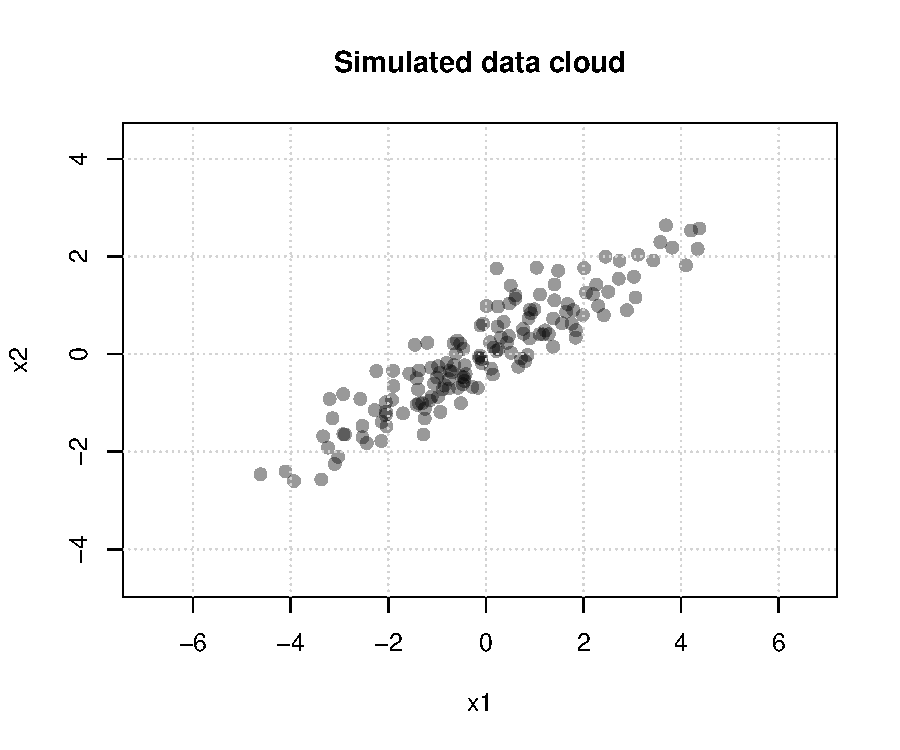
\includegraphics[width=0.6\textwidth]{img/pca-scatter.pdf}
  \caption{The simulated data cloud.}
\end{figure}

\subsection{Interpretation of the scatter plot}

This graph is the starting point. PCA is a \textbf{geometric} method, so we first look at the
\emph{shape} of the data cloud: if the cloud is \textbf{elongated}, most of the variation may lie close
to one direction. PCA formalizes that intuition.

\subsection{Covariance matrix and spectral decomposition}

We center the data and compute $S = \frac{1}{n}X_c^\top X_c$, then its eigen-decomposition:

\begin{lstlisting}
X_centered <- scale(X, center = TRUE, scale = FALSE)   # X_c: subtract column means
S <- crossprod(X_centered) / nrow(X_centered)          # crossprod(A) = t(A) %*% A

S
##          x1       x2
## x1 3.584051 2.004268
## x2 2.004268 1.334890

eig <- eigen(S)
eig$values
## [1] 4.757681 0.161260
eig$vectors
##            [,1]       [,2]
## [1,] -0.8629393  0.5053075
## [2,] -0.5053075 -0.8629393
\end{lstlisting}

\esempio{
  Reading the output with the theory:
  \begin{itemize}
    \item $S_{11} \approx 3.58$ and $S_{22} \approx 1.33$ are the variances; $S_{12} \approx 2.00 > 0$:
          $x_1$ and $x_2$ grow together (correlation $2.00/\sqrt{3.58 \cdot 1.33} \approx 0.92$);
    \item $\lambda_1 \approx 4.76$, $\lambda_2 \approx 0.16$: almost all variance is along $\bs{p}_1$;
    \item the columns of \texttt{eig\$vectors} are $\bs{p}_1, \bs{p}_2$: unit length and orthogonal;
    \item check: $\lambda_1 + \lambda_2 = 4.918941 = S_{11} + S_{22} = \operatorname{tr}(S)$.
  \end{itemize}
}

\osservazione{
  \textbf{Sign of eigenvectors.} If $\bs{p}$ is a unit eigenvector, so is $-\bs{p}$. Here R returns
  $\bs{p}_1 = (-0.86, -0.51)^\top$, but $(0.86, 0.51)^\top$ is equally valid. So principal directions
  and scores are defined only \emph{up to sign}.
}

\osservazione{
  \textbf{$n$ vs $n-1$ again.} Here $S$ uses denominator $n$. By contrast, \texttt{prcomp()} reports
  component variances with denominator $n-1$ (R's sample-covariance convention). This multiplies the
  eigenvalues by $n/(n-1)$ but does \red{not} change the principal directions, the latent scores
  (up to sign), the reconstructions or the explained-variance ratios.
}

\subsection{Principal directions}

We draw each principal direction as an arrow:

\begin{lstlisting}
mu     <- colMeans(X)
P      <- eig$vectors
lambda <- eig$values

arrows_df <- data.frame(
  x0 = mu[1], y0 = mu[2],
  x1 = mu[1] + 2 * sqrt(lambda[1]) * P[1, 1],
  y1 = mu[2] + 2 * sqrt(lambda[1]) * P[2, 1],
  x2 = mu[1] + 2 * sqrt(lambda[2]) * P[1, 2],
  y2 = mu[2] + 2 * sqrt(lambda[2]) * P[2, 2]
)
##             x0        y0        x1        y1        x2         y2
## x1 -0.04872574 0.0173874 -3.813231 -2.186977 0.3571088 -0.6756769
\end{lstlisting}

(then plotted with \texttt{ggplot2}: \texttt{geom\_point} for the data and one \texttt{geom\_segment}
with an arrow for each direction.)

\begin{figure}[H]
  \centering
  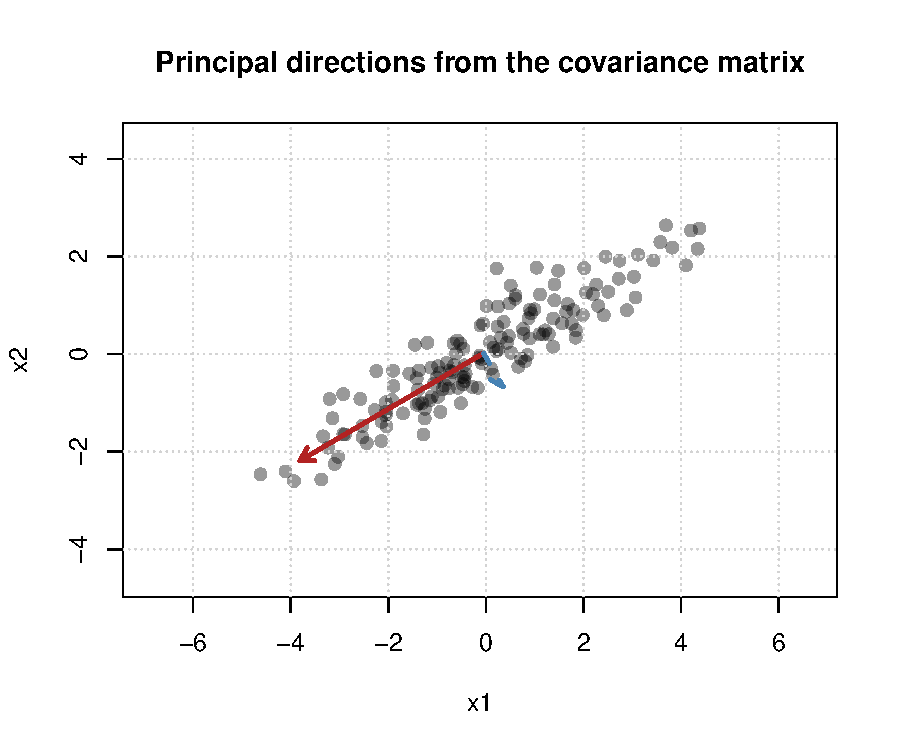
\includegraphics[width=0.6\textwidth]{img/pca-directions.pdf}
  \caption{First principal direction (solid, red) and second (dashed, blue).}
\end{figure}

\subsubsection{Interpretation}

Each arrow is
\[
  \underbrace{\mu}_{\text{start}} \;+\; \underbrace{2\sqrt{\lambda_j}}_{\text{length}} \; \underbrace{\bs{p}_j}_{\text{direction}},
  \qquad\text{i.e.\ in R:}\quad \texttt{mu + 2 * sqrt(lambda[j]) * P[, j]}.
\]
\begin{itemize}
  \item \textbf{start}: the empirical mean $\mu = \frac{1}{n}\sum_{i} x_i$, the center of the cloud;
        this is why both arrows start at \texttt{(mu[1], mu[2])};
  \item \textbf{direction}: the eigenvector, \texttt{P[, 1]} for the first principal direction and
        \texttt{P[, 2]} for the second;
  \item \textbf{length}: $\lambda_j$ is the \emph{variance} along $\bs{p}_j$, so $\sqrt{\lambda_j}$ is a
        \emph{standard deviation}, which has the same units as the data. The factor $2$ is only a
        visualization choice to make the arrows clearly visible.
\end{itemize}

\subsection{Explained variance ratio}

\begin{lstlisting}
prop_var <- eig$values / sum(eig$values)
\end{lstlisting}

\begin{center}
\begin{tabular}{ccc}
  \hline
  Component & Eigenvalue & Explained variance ratio \\
  \hline
  1 & 4.7577 & 0.9672 \\
  2 & 0.1613 & 0.0328 \\
  \hline
\end{tabular}
\end{center}

In this example \textbf{one component already explains $96.7\%$ of the variability}: with $q = 1$,
$V_1 = \lambda_1$ and the lost variance is only $J_1 = \lambda_2$.

\subsection{Projection and reconstruction}

With one retained component, each observation is projected onto the line through $\mu$ spanned by
the first principal direction.

\dfn{Score and reconstruction ($q = 1$)}{
  The \emph{score} of observation $i$ on the first component and its \emph{reconstruction} are
  \[
    z_i = \bs{p}_1^\top (x_i - \mu), \qquad
    \hat{x}_i = \mu + z_i\, \bs{p}_1 = \mu + \bs{p}_1 \bs{p}_1^\top (x_i - \mu).
  \]
  The \emph{reconstruction error} is the vector $x_i - \hat{x}_i$.
}

We compute this with \texttt{prcomp()}, where \texttt{\$x} are the scores $z_i$, \texttt{\$rotation} the
loadings (the matrix $P$) and \texttt{\$center} the mean $\mu$:

\begin{lstlisting}
pca_fit <- prcomp(X, center = TRUE, scale. = FALSE)

scores1   <- pca_fit$x[, 1, drop = FALSE]          # z_i         (n x 1)
loadings1 <- pca_fit$rotation[, 1, drop = FALSE]   # p_1         (2 x 1)

Xhat1 <- scores1 %*% t(loadings1)                  # z_i p_1^T   (n x 2)
Xhat1 <- sweep(Xhat1, 2, pca_fit$center, "+")      # add mu back to each row

head(data.frame(x1 = X[, 1], x2 = X[, 2],
                x1_hat = Xhat1[, 1], x2_hat = Xhat1[, 2]))
##           x1          x2      x1_hat      x2_hat
## 1 -1.1209513 -0.27870135 -0.97628325 -0.52575832
## 2 -0.4603550  0.10830813 -0.31560537 -0.13888812
## 3  3.1174166  2.03655127  3.18944333  1.91354762
## 4  0.1410168 -0.41957823 -0.09797001 -0.01144835
## 5  0.2585755  0.09541898  0.21413615  0.17131026
## 6  3.4301300  1.91788032  3.37056335  2.01960526
\end{lstlisting}

\begin{figure}[H]
  \centering
  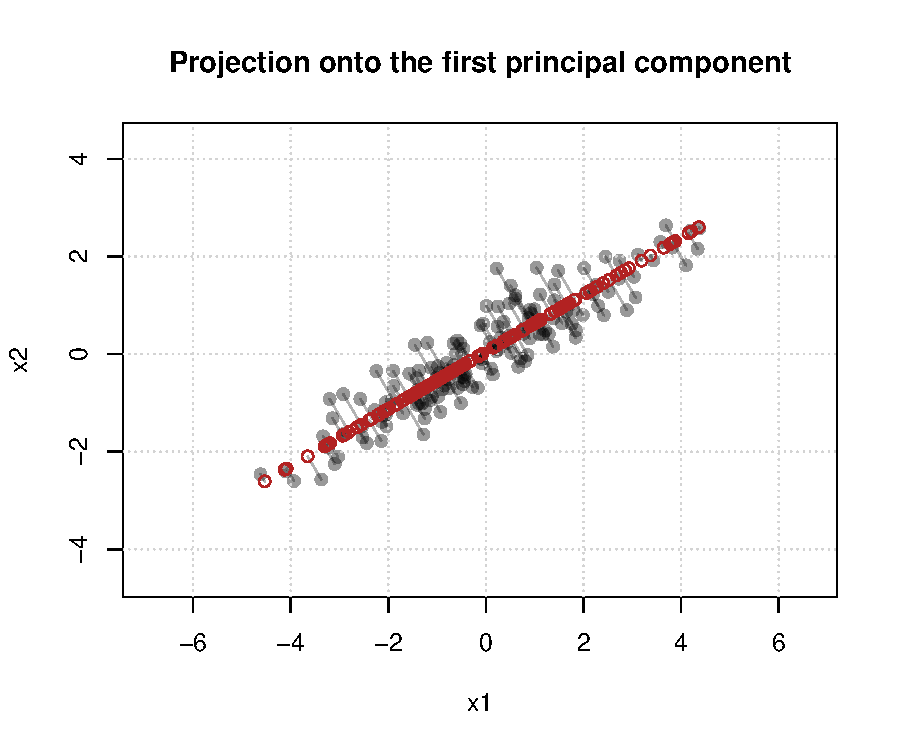
\includegraphics[width=0.6\textwidth]{img/pca-reconstruction.pdf}
  \caption{Original points (black), reconstructions $\hat{x}_i$ (red circles) and reconstruction errors (segments).}
\end{figure}

\subsubsection{Interpretation}

There are three geometric objects in this figure:
\begin{itemize}
  \item the \textbf{original data points} $x_i$ (\texttt{x1, x2});
  \item the \textbf{reconstructed points} $\hat{x}_i$ (\texttt{x1\_hat, x2\_hat}): the projections of the
        original observations onto the first principal component, so they all lie on one line;
  \item the \textbf{segments} between them, each representing the reconstruction error $x_i - \hat{x}_i$.
\end{itemize}
This is why the graph is useful: it shows visually what PCA does when only one component is kept.

\osservazione{
  The segments are \textbf{perpendicular} to the line: $x_i - \hat{x}_i$ is the component of $x_i - \mu$
  along $\bs{p}_2$. Hence the average squared length of the segments is exactly the lost variance:
  \[
    \frac{1}{n}\sum_{i=1}^{n} \|x_i - \hat{x}_i\|^2 = \lambda_2 = J_1 \approx 0.16.
  \]
  Maximizing the variance kept is the same as minimizing the reconstruction error.
}

\section{Choosing the Dimension of the Projection Subspace}

As before, the data are \textbf{centered}, so projections pass through the origin.

\subsection{Projection and reconstruction error}

\dfn{Projection onto a $q$-dimensional subspace}{
  Let $P_q = [\,\bs{p}_1 \mid \cdots \mid \bs{p}_q\,] \in \mathbb{R}^{p \times q}$ have
  \textbf{orthonormal columns}, i.e.\ an orthonormal basis of a $q$-dimensional subspace.
  The projection of $x_i$ onto that subspace is
  \[
    \tilde{x}_i = P_q P_q^\top x_i
    = \sum_{j=1}^{q} (\bs{p}_j^\top x_i)\, \bs{p}_j .
  \]
  Read right to left: $P_q^\top x_i \in \mathbb{R}^q$ are the $q$ scores (coordinates in the basis),
  and multiplying by $P_q$ maps them back to $\mathbb{R}^p$.
}

\mprop{Properties of $P_q$}{
  \begin{enumerate}
    \item $P_q^\top P_q = I_q$;
    \item $P_q P_q^\top$ is an \textbf{orthogonal projector}:
          \[
            (P_q P_q^\top)^\top = P_q P_q^\top \quad\text{(symmetric)}, \qquad
            (P_q P_q^\top)^2 = P_q P_q^\top \quad\text{(idempotent)}.
          \]
  \end{enumerate}
}

\pf{Proof}{
  \begin{enumerate}
    \item The $(j,k)$ entry of $P_q^\top P_q$ is $\bs{p}_j^\top \bs{p}_k$, which is $1$ if $j = k$ and $0$
          otherwise, by orthonormality.
    \item $(P_q P_q^\top)^\top = (P_q^\top)^\top P_q^\top = P_q P_q^\top$, and
          $(P_q P_q^\top)(P_q P_q^\top) = P_q \underbrace{(P_q^\top P_q)}_{I_q} P_q^\top = P_q P_q^\top$.
  \end{enumerate}
}

\osservazione{
  Idempotent means ``projecting twice = projecting once'': a point already in the subspace does not move.
  Note that $P_q P_q^\top \neq I_p$ when $q < p$ (it is a $p \times p$ matrix of rank $q$),
  while $P_q^\top P_q = I_q$ always.
}

\teorema{
  For every $P_q$ with orthonormal columns, the average squared reconstruction error is
  \[
    \frac{1}{n}\sum_{i=1}^{n} \|x_i - \tilde{x}_i\|^2 = \operatorname{tr}(S) - \operatorname{tr}(P_q^\top S P_q).
  \]
  Hence \textbf{minimizing the reconstruction error} and \textbf{maximizing the explained variance}
  $\operatorname{tr}(P_q^\top S P_q)$ are the \red{same problem}. The minimum is attained by the first $q$
  eigenvectors of $S$, and equals the lost variance:
  \[
    J_{p-q} = \sum_{j=q+1}^{p} \lambda_j = \frac{1}{n}\sum_{i=1}^{n} \|x_i - \tilde{x}_i\|^2 .
  \]
}

\pf{Proof}{
  Let $\Pi = P_q P_q^\top$. By the previous proposition, $x_i - \tilde{x}_i = (I - \Pi)x_i$ is orthogonal
  to $\tilde{x}_i = \Pi x_i$ (since $\Pi^\top (I - \Pi) = \Pi - \Pi^2 = 0$), so by Pythagoras
  \[
    \|x_i - \tilde{x}_i\|^2 = \|x_i\|^2 - \|\tilde{x}_i\|^2 = \|x_i\|^2 - \|P_q^\top x_i\|^2 ,
  \]
  where $\|\tilde{x}_i\|^2 = x_i^\top P_q P_q^\top P_q P_q^\top x_i = \|P_q^\top x_i\|^2$.
  Averaging over $i$ (data centered, $S = \frac{1}{n}\sum_i x_i x_i^\top$):
  \[
    \frac{1}{n}\sum_i \|x_i\|^2 = \operatorname{tr}(S), \qquad
    \frac{1}{n}\sum_i \|P_q^\top x_i\|^2 = \operatorname{tr}(P_q^\top S P_q).
  \]
  By the ``best $q$-dimensional subspace'' theorem, $\operatorname{tr}(P_q^\top S P_q) \leq \lambda_1 + \dots + \lambda_q$,
  with equality for the first $q$ eigenvectors. So the minimal error is
  $\operatorname{tr}(S) - (\lambda_1 + \dots + \lambda_q) = \lambda_{q+1} + \dots + \lambda_p = J_{p-q}$.
}

\osservazione{
  This is exactly what we saw in the R example: with $q = 1$ the average squared length of the
  segments was $\lambda_2 \approx 0.16 = J_1$.
}

\begin{Exercise}{Suggested exercise 28}{}
  Let $S = P\Lambda P^\top$ with orthonormal eigenvectors $P = [\bs{p}_1, \dots, \bs{p}_p]$ and
  $\lambda_1 \geq \dots \geq \lambda_p \geq 0$. For $q \leq p$ let $P_q = [\bs{p}_1, \dots, \bs{p}_q]$.
  Show that $\Pi_q := P_q P_q^\top$ is an orthogonal projector.
\end{Exercise}

\pf{Solution}{
  An orthogonal projector is a matrix that is \textbf{symmetric} and \textbf{idempotent}.
  \begin{itemize}
    \item Symmetry: $\Pi_q^\top = (P_q P_q^\top)^\top = (P_q^\top)^\top P_q^\top = P_q P_q^\top = \Pi_q$.
    \item Idempotence: $\Pi_q^2 = P_q (P_q^\top P_q) P_q^\top = P_q I_q P_q^\top = \Pi_q$.
  \end{itemize}
  Moreover it projects onto $\operatorname{span}(\bs{p}_1, \dots, \bs{p}_q)$:
  $\Pi_q \bs{p}_k = \sum_{j \leq q} \bs{p}_j (\bs{p}_j^\top \bs{p}_k)$ equals $\bs{p}_k$ if $k \leq q$ and $0$ if $k > q$.
  The residual is orthogonal to the image: $\Pi_q^\top (I - \Pi_q) = \Pi_q - \Pi_q^2 = 0$.
}

\begin{Exercise}{Suggested exercise 29}{}
  Let $x_1, \dots, x_n \in \mathbb{R}^p$ be centered, $S = \frac{1}{n}\sum_i x_i x_i^\top$ with eigenvalues
  $\lambda_1 \geq \dots \geq \lambda_p \geq 0$ and orthonormal eigenvectors $\bs{p}_1, \dots, \bs{p}_p$.
  Let $P_q = [\bs{p}_1, \dots, \bs{p}_q]$ and $\tilde{x}_i = P_q P_q^\top x_i$. Show that
  \[
    J_{p-q} = \sum_{j=q+1}^{p} \lambda_j = \frac{1}{n}\sum_{i=1}^{n} \|x_i - \tilde{x}_i\|^2 .
  \]
\end{Exercise}

\pf{Solution}{
  (A direct proof, alternative to the one of the theorem above.) Expand $x_i$ in the orthonormal basis of eigenvectors:
  $x_i = \sum_{j=1}^{p} (\bs{p}_j^\top x_i)\, \bs{p}_j$, while $\tilde{x}_i = \sum_{j \leq q} (\bs{p}_j^\top x_i)\, \bs{p}_j$. Then
  \[
    x_i - \tilde{x}_i = \sum_{j=q+1}^{p} (\bs{p}_j^\top x_i)\, \bs{p}_j
    \quad\Longrightarrow\quad
    \|x_i - \tilde{x}_i\|^2 = \sum_{j=q+1}^{p} (\bs{p}_j^\top x_i)^2
  \]
  (Pythagoras in an orthonormal basis). Averaging over $i$,
  \[
    \frac{1}{n}\sum_i \|x_i - \tilde{x}_i\|^2
    = \sum_{j=q+1}^{p} \bs{p}_j^\top \Big( \frac{1}{n}\sum_i x_i x_i^\top \Big) \bs{p}_j
    = \sum_{j=q+1}^{p} \bs{p}_j^\top S \bs{p}_j = \sum_{j=q+1}^{p} \lambda_j ,
  \]
  since $\bs{p}_j^\top S \bs{p}_j = \lambda_j \bs{p}_j^\top \bs{p}_j = \lambda_j$.
}

\subsection{How many components should we keep?}

A practical question in PCA: \textbf{how large should $q$ be?}
\begin{itemize}
  \item \textbf{too few} components: we may lose important structure in the data;
  \item \textbf{too many} components: we keep noise and lose the benefit of dimensionality reduction.
\end{itemize}

Recall that the eigenvalues of $S$ measure how much variance each principal direction explains,
and the \textbf{total variance} of the data is
\[
  \operatorname{tr}(S) = \sum_{j=1}^{p} \lambda_j .
\]

\dfn{Rank-$q$ covariance and proportion of explained variance}{
  Let $\Lambda_q = \operatorname{diag}(\lambda_1, \dots, \lambda_q)$ and
  \[
    \tilde{S}_q = P_q \Lambda_q P_q^\top \in \mathbb{R}^{p \times p},
  \]
  i.e.\ the spectral decomposition $S = P\Lambda P^\top$ truncated to the first $q$ terms:
  $\tilde{S}_q = \sum_{j=1}^{q} \lambda_j \bs{p}_j \bs{p}_j^\top$ (it is the covariance of the projected data $\tilde{x}_i$).
  The \emph{cumulative proportion of explained variance} is
  \[
    \mathrm{PEV}(q) = \frac{\operatorname{tr}(\tilde{S}_q)}{\operatorname{tr}(S)}
    = \frac{\sum_{j=1}^{q} \lambda_j}{\sum_{j=1}^{p} \lambda_j} \in [0, 1].
  \]
}

\osservazione{
  Why $\operatorname{tr}(\tilde{S}_q) = \sum_{j \leq q} \lambda_j$: by the cyclic property of the trace,
  $\operatorname{tr}(P_q \Lambda_q P_q^\top) = \operatorname{tr}(\Lambda_q P_q^\top P_q) = \operatorname{tr}(\Lambda_q)$.
  $\mathrm{PEV}(q)$ is increasing in $q$, with $\mathrm{PEV}(p) = 1$.
}

\dfn{Threshold criterion}{
  Fix a threshold $\tau$ (typically $\tau = 0.80$, $0.90$ or $0.95$) and choose
  \[
    q^* = \min\{\, q : \mathrm{PEV}(q) \geq \tau \,\},
  \]
  the \textbf{smallest} number of components explaining at least a fraction $\tau$ of the total variance.
}

\dfn{Scree plot}{
  The \emph{scree plot} displays the individual eigenvalues $\lambda_j$ (or the explained-variance ratios
  $\lambda_j / \operatorname{tr}(S)$) against the component index $j$. One looks for an \textbf{elbow}:
  \begin{itemize}
    \item \textbf{before} the elbow, eigenvalues decrease quickly: components usually considered \emph{important};
    \item \textbf{after} the elbow, they flatten out: components often interpreted as mostly \emph{noise}
          or weak structure.
  \end{itemize}
}

\esempio{
  Suppose $p = 7$ with eigenvalues $6,\ 3,\ 1.2,\ 0.4,\ 0.3,\ 0.2,\ 0.1$, so $\operatorname{tr}(S) = 11.2$.

  \begin{center}
  \begin{tabular}{c|ccccccc}
    $q$ & 1 & 2 & 3 & 4 & 5 & 6 & 7 \\
    \hline
    $\mathrm{PEV}(q)$ & 0.536 & 0.804 & 0.911 & 0.946 & 0.973 & 0.991 & 1
  \end{tabular}
  \end{center}

  \begin{itemize}
    \item $\tau = 0.80$: $q^* = 2$;
    \item $\tau = 0.90$: $q^* = 3$;
    \item $\tau = 0.95$: $q^* = 5$ (since $\mathrm{PEV}(4) = 0.946 < 0.95$).
  \end{itemize}

  \begin{center}
    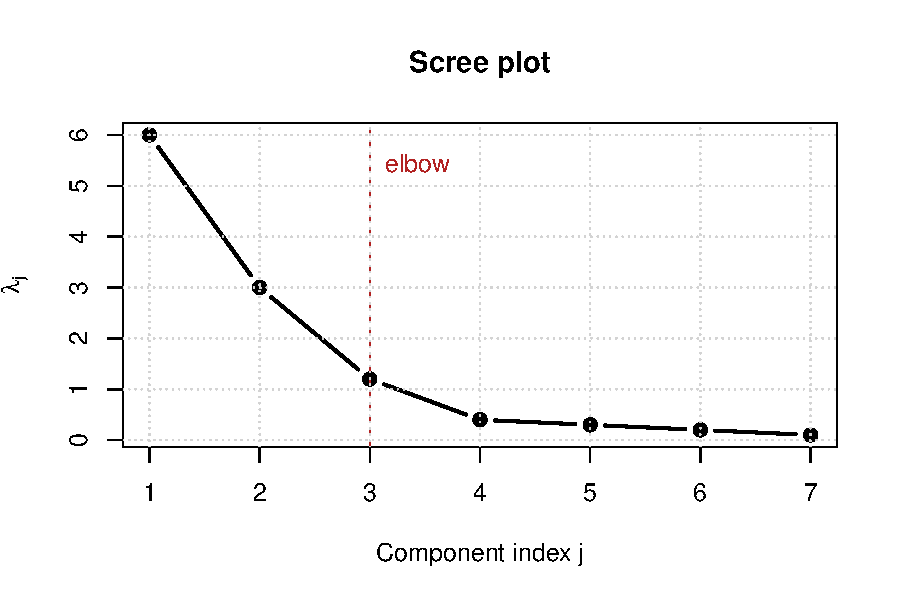
\includegraphics[width=0.6\textwidth]{img/pca-scree.pdf}
  \end{center}

  The scree plot drops fast up to $j = 3$ and is almost flat afterwards: the elbow suggests $q = 3$.
  Different criteria can give different answers, so the choice of $q$ is partly a judgment call.

  In the R example of the previous section, $\mathrm{PEV}(1) = 0.967$: $q = 1$ already satisfies all
  three thresholds.
}

\subsection{Practical workflow for choosing $q$}

In practice, a reasonable workflow is:
\begin{enumerate}
  \item compute the PCA;
  \item inspect the scree plot;
  \item inspect the cumulative explained variance curve;
  \item choose a first candidate value of $q$;
  \item check whether that value is appropriate for the intended purpose.
\end{enumerate}

The best value of $q$ \textbf{depends on the goal}:
\begin{itemize}
  \item for \textbf{visualization}, one often takes $q = 2$ or $q = 3$;
  \item for \textbf{compression}, one takes the smallest $q$ giving an acceptable reconstruction quality;
  \item for \textbf{preprocessing in machine learning}, one may choose $q$ based on the downstream predictive performance.
\end{itemize}
So the choice of $q$ combines statistical criteria, interpretability and the final objective of the analysis.

\subsection{Illustration in R}

We simulate $n = 200$ observations of $p = 5$ variables driven by three latent factors $z_1, z_2, z_3$
with standard deviations $3$, $1.5$, $0.5$: $x_1, x_2$ depend on $z_1$, $x_3, x_4$ on $z_2$, $x_5$ on $z_3$,
each plus a small noise ($\mathrm{sd} = 0.2$).

\begin{lstlisting}
set.seed(123)
n  <- 200
z1 <- rnorm(n, sd = 3); z2 <- rnorm(n, sd = 1.5); z3 <- rnorm(n, sd = 0.5)
x1 <- z1 + rnorm(n, sd = 0.2)
x2 <- 0.8 * z1 + rnorm(n, sd = 0.2)
x3 <- z2 + rnorm(n, sd = 0.2)
x4 <- 0.7 * z2 + rnorm(n, sd = 0.2)
x5 <- z3 + rnorm(n, sd = 0.2)
X  <- scale(cbind(x1, x2, x3, x4, x5), center = TRUE, scale = FALSE)

pca <- prcomp(X, center = FALSE, scale. = FALSE)
eigenvalues <- pca$sdev^2
eigenvalues
## [1] 13.06986281  3.37695148  0.28067228  0.04648912  0.03056518
screeplot(pca, type = "lines", main = "Scree Plot from prcomp")

pev     <- eigenvalues / sum(eigenvalues)
cum_pev <- cumsum(pev)
\end{lstlisting}

Since \texttt{prcomp()} uses the $n-1$ convention, these eigenvalues are on a slightly different scale
from those computed with denominator $n$; the explained-variance ratios are unaffected.

\begin{center}
\begin{tabular}{cccc}
  \hline
  Component & Eigenvalue & Explained variance ratio & Cumulative \\
  \hline
  1 & 13.0699 & 0.7778 & 0.7778 \\
  2 &  3.3770 & 0.2010 & 0.9787 \\
  3 &  0.2807 & 0.0167 & 0.9954 \\
  4 &  0.0465 & 0.0028 & 0.9982 \\
  5 &  0.0306 & 0.0018 & 1.0000 \\
  \hline
\end{tabular}
\end{center}

\begin{figure}[H]
  \centering
  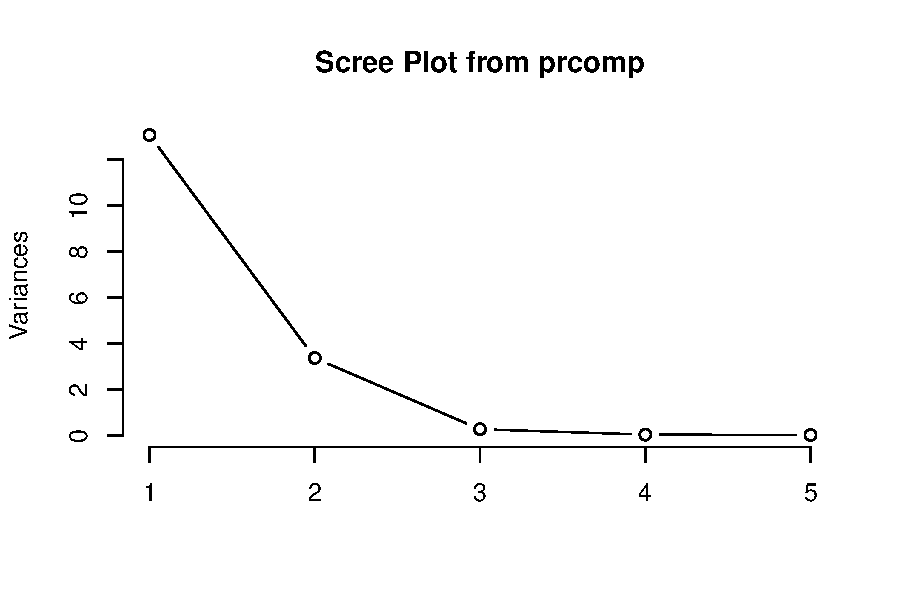
\includegraphics[width=0.48\textwidth]{img/pca5-scree.pdf}\hfill
  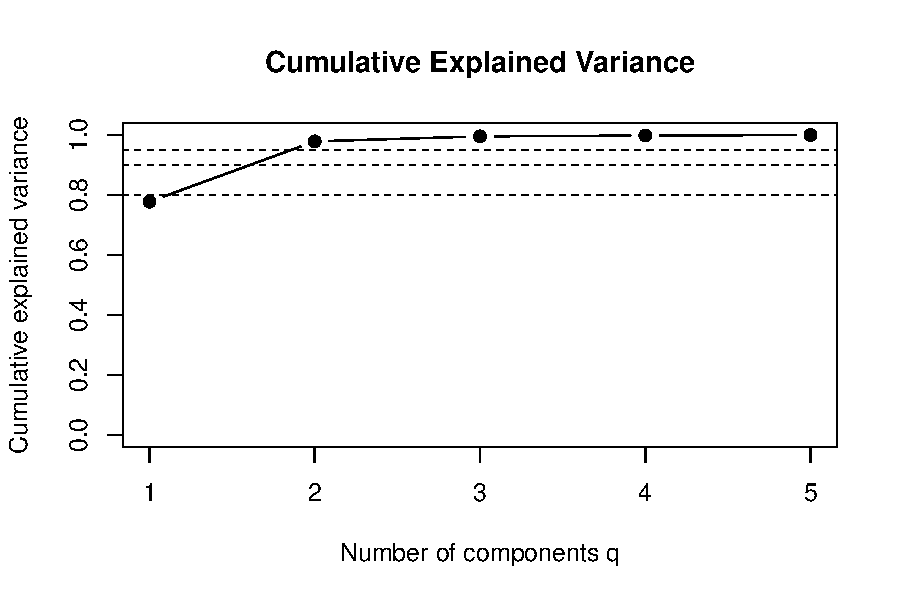
\includegraphics[width=0.48\textwidth]{img/pca5-cumvar.pdf}
  \caption{Scree plot and cumulative explained variance (dashed lines: $\tau = 0.80, 0.90, 0.95$).}
\end{figure}

\esempio{
  Reading the output:
  \begin{itemize}
    \item threshold criterion: $\mathrm{PEV}(1) = 0.778 < 0.80$, while $\mathrm{PEV}(2) = 0.979$ is above
          all three thresholds, so $q^* = 2$ for $\tau = 0.80, 0.90, 0.95$;
    \item scree plot: big drop from $\lambda_2$ to $\lambda_3$, then flat: the elbow also gives $q = 2$;
    \item this matches the simulation: two \emph{strong} latent factors. The variance carried by $z_1$ through
          $(x_1, x_2)$ is about $9\,(1 + 0.8^2) = 14.8$ and by $z_2$ through $(x_3, x_4)$ about $2.25\,(1 + 0.7^2) = 3.35$,
          close to $\lambda_1, \lambda_2$; $\lambda_3 \approx 0.28 \approx 0.5^2 + 0.2^2$ is the weak factor $z_3$ in $x_5$,
          and $\lambda_4, \lambda_5 \approx 0.04 = 0.2^2$ are pure noise.
  \end{itemize}
}

\section{Projection into the Latent Space}

It is important to distinguish \textbf{three objects}:
\begin{itemize}
  \item the \textbf{original observations} $x_i$, in the variable space $\mathbb{R}^p$;
  \item the \textbf{latent scores}, the coordinates in the PCA space $\mathbb{R}^q$:
        \[
          Z = XP_q \in \mathbb{R}^{n \times q};
        \]
  \item the \textbf{reconstructed observations}, mapped back to the original variable space:
        \[
          \hat{X} = Z P_q^\top = X P_q P_q^\top \in \mathbb{R}^{n \times p}.
        \]
\end{itemize}

\mprop{The latent scores are uncorrelated}{
  The columns of $Z = XP_q$ have mean zero, variances $\lambda_1, \dots, \lambda_q$ and are pairwise uncorrelated:
  \[
    \frac{1}{n} Z^\top Z = \Lambda_q = \operatorname{diag}(\lambda_1, \dots, \lambda_q).
  \]
}

\pf{Proof}{
  Mean: $\frac{1}{n}\mathbf{1}_n^\top Z = \big(\frac{1}{n}\mathbf{1}_n^\top X\big) P_q = 0$ because $X$ is centered.
  Covariance: $\frac{1}{n}Z^\top Z = P_q^\top \big(\frac{1}{n}X^\top X\big) P_q = P_q^\top S P_q$.
  Since $S\bs{p}_j = \lambda_j\bs{p}_j$, we have $SP_q = P_q\Lambda_q$, hence $P_q^\top S P_q = P_q^\top P_q \Lambda_q = \Lambda_q$.
}

\osservazione{
  So PCA is a \textbf{rotation} of the data (for $q = p$, $Z = XP$ with $P$ orthogonal) to new coordinates that are
  uncorrelated and ordered by decreasing variance.
}

\subsection{Loadings}

\dfn{Loading vectors}{
  The eigenvectors $\bs{p}_1, \dots, \bs{p}_p$ of $S = P\Lambda P^\top$ are also called \emph{loading vectors}: they give the
  principal directions, while the eigenvalues measure the variance explained along them.
}

Keeping the first two directions, $P_2 = [\bs{p}_1, \bs{p}_2] \in \mathbb{R}^{p \times 2}$ and $Z_2 = XP_2 \in \mathbb{R}^{n \times 2}$:
the rows of $Z_2$ are the coordinates of the observations in the two-dimensional PCA space. By
Suggested exercise 23,
\[
  \bs{z}_i = x_i^\top P_2 = \sum_{j=1}^{p} x_{ij} \begin{bmatrix} p_{j1} & p_{j2} \end{bmatrix},
\]
so the \textbf{row} $(p_{j1}, p_{j2})$ of $P_2$ contains the two coefficients of variable $j$ in the first two
principal directions:
\begin{itemize}
  \item if $|p_{j1}|$ is large, variable $j$ receives a large weight in PC1 (similarly for $|p_{j2}|$ and PC2);
  \item the \textbf{signs} tell whether variables enter a component in the same or in opposite directions.
\end{itemize}
Coefficient magnitudes are directly comparable only when the variables have comparable units or have been
\textbf{standardized}.

\mprop{Correlation coordinates}{
  Let $s_j$ be the standard deviation of variable $j$. The correlation between variable $j$ and the $k$-th latent
  score is
  \[
    \operatorname{cor}(x_{\cdot j}, z_{\cdot k}) = \frac{\sqrt{\lambda_k}\, p_{jk}}{s_j}.
  \]
  The pair $\big( \sqrt{\lambda_1}\,p_{j1}/s_j,\; \sqrt{\lambda_2}\,p_{j2}/s_j \big)$ is called the
  \emph{correlation coordinates} of variable $j$.
}

\pf{Proof}{
  Data are centered, so (with the same denominator $n$ everywhere)
  \[
    \operatorname{cov}(x_{\cdot j}, z_{\cdot k}) = \frac{1}{n}\sum_i x_{ij}\, (x_i^\top \bs{p}_k)
    = \Big( \frac{1}{n}\sum_i x_i x_i^\top \bs{p}_k \Big)_j = (S\bs{p}_k)_j = \lambda_k\, p_{jk}.
  \]
  By the previous proposition $\operatorname{var}(z_{\cdot k}) = \lambda_k$, hence
  \[
    \operatorname{cor}(x_{\cdot j}, z_{\cdot k}) = \frac{\lambda_k\, p_{jk}}{s_j\sqrt{\lambda_k}} = \frac{\sqrt{\lambda_k}\, p_{jk}}{s_j}. \qedhere
  \]
}

\osservazione{
  Summing over all components, $\sum_{k=1}^{p} \operatorname{cor}(x_{\cdot j}, z_{\cdot k})^2 = \frac{1}{s_j^2}\sum_k \lambda_k p_{jk}^2 = \frac{S_{jj}}{s_j^2} = 1$
  (because $S_{jj} = (P\Lambda P^\top)_{jj} = \sum_k \lambda_k p_{jk}^2$). So the squared length of the correlation-coordinate
  arrow in the PC1--PC2 plane is the fraction of the variance of variable $j$ captured by the first two components: it is
  at most $1$, and close to $1$ when the variable is well represented in the plane.
}

\subsection{Biplot}

\dfn{Biplot}{
  A \emph{biplot} is the joint representation of observations and variables in the plane of two principal components:
  \begin{itemize}
    \item \textbf{observation points}: each row of $Z_2$ is plotted as a point;
    \item \textbf{variable arrows}: each original variable is an arrow, based on its coordinates in the loading matrix.
  \end{itemize}
  Often several biplots are used (PC1--PC2, PC1--PC3, \dots).
}

The exact interpretation depends on the scaling convention. In a latent score plot with
correlation-coordinate arrows:
\begin{itemize}
  \item observations close to each other have similar latent scores; observations far apart differ strongly along the
        displayed components; \textbf{clusters} may reveal structure;
  \item a \textbf{long} arrow means the variable is well represented in the PC1--PC2 plane; a \textbf{short} arrow means
        a substantial part of its variation lies in later components;
  \item arrows pointing in \textbf{similar} directions: positively associated variables; \textbf{opposite} directions:
        negatively associated; close to \textbf{orthogonal}: weak association in the displayed plane;
  \item the \textbf{angle} between arrows approximates the correlation between the variables, when the plane represents them well;
  \item an observation lying far in the direction of an arrow tends to have a relatively \textbf{large} value of that
        variable; in the opposite direction, a relatively \textbf{small} value.
\end{itemize}

\osservazione{
  In practice arrows are often rescaled for visibility: one plots $c\,[\,p_{j1}\ p_{j2}\,]$ for some $c > 0$. This changes the
  visual length but not the direction; after an arbitrary rescaling, the arrow length \red{must not} be read as a
  correlation or as a quality of representation. When using a biplot:
  \begin{itemize}
    \item always check the explained variance of PC1 and PC2;
    \item standardize variables if they are on very different scales;
    \item avoid over-interpreting tiny differences in arrow lengths;
    \item use it together with scree plots and explained-variance summaries.
  \end{itemize}
}

\section{PCA of Iris Data}

The \texttt{iris} dataset (150 flowers, 3 species, 4 measurements in cm) is a classical PCA example.

\begin{lstlisting}
data(iris)
X       <- iris[, 1:4]
species <- iris$Species
pca_iris <- prcomp(X, center = TRUE, scale. = TRUE)
summary(pca_iris)
## Importance of components:
##                           PC1    PC2     PC3     PC4
## Standard deviation     1.7084 0.9560 0.38309 0.14393
## Proportion of Variance 0.7296 0.2285 0.03669 0.00518
## Cumulative Proportion  0.7296 0.9581 0.99482 1.00000
pca_iris$rotation[, 1:2]
##                     PC1         PC2
## Sepal.Length  0.5210659 -0.37741762
## Sepal.Width  -0.2693474 -0.92329566
## Petal.Length  0.5804131 -0.02449161
## Petal.Width   0.5648565 -0.06694199
biplot(pca_iris, cex = 0.6)
\end{lstlisting}

\osservazione{
  \textbf{Standardization.} With \texttt{scale. = TRUE} every variable is divided by its standard deviation, so $S$ becomes
  the \textbf{correlation matrix} $R$ ($R_{jj} = 1$). Then the total variance is $\operatorname{tr}(R) = p = 4$, and indeed
  $1.7084^2 / 4 = 2.919/4 = 0.7296$. Standardizing prevents a variable from dominating only because of its unit of measurement.
}

\begin{figure}[H]
  \centering
  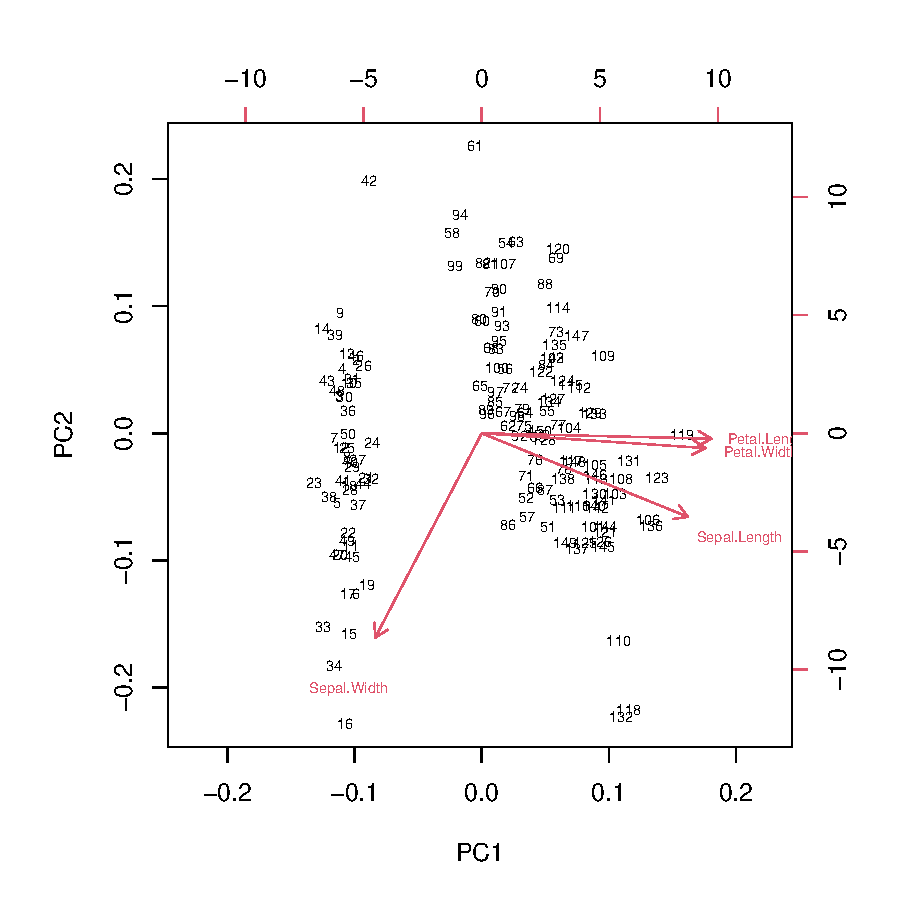
\includegraphics[width=0.48\textwidth]{img/iris-biplot.pdf}\hfill
  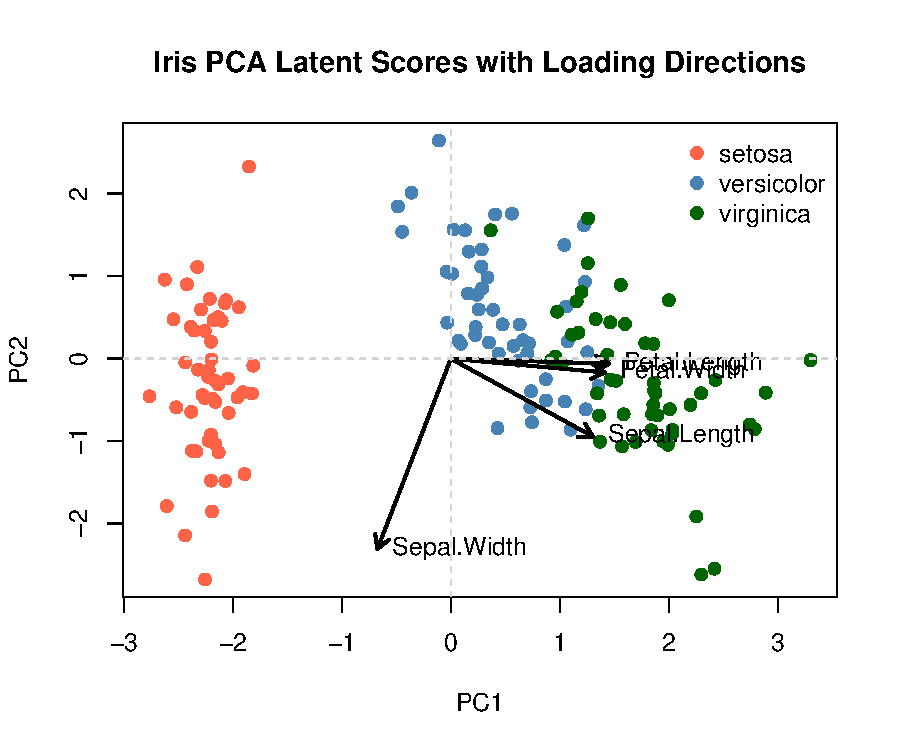
\includegraphics[width=0.48\textwidth]{img/iris-colored.pdf}
  \caption{Standard \texttt{biplot()} and a colored manual version (scores coloured by species, loading arrows scaled by $2.5$).}
\end{figure}

The colored version is built from \texttt{scores <- pca\_iris\$x[, 1:2]} and \texttt{loadings <- pca\_iris\$rotation[, 1:2]},
with \texttt{arrows(0, 0, 2.5 * loadings[, 1], 2.5 * loadings[, 2])}.

\esempio{
  \begin{itemize}
    \item PC1 and PC2 explain $95.8\%$ of the variance: the plane is a faithful summary.
    \item PC1 has loadings $\approx 0.58$ and $0.56$ on petal length and width and $0.52$ on sepal length: it is roughly an
          average of them, i.e.\ a \textbf{flower (petal) size} component. Sepal width enters with the opposite sign.
    \item PC2 is dominated by sepal width ($-0.92$).
    \item The three species are well separated along PC1 alone: \emph{setosa} (small petals) on one side,
          \emph{versicolor} and \emph{virginica} on the other.
  \end{itemize}
}

% =====================================================================
\section{PCA in High-Dimensional Settings}

\subsection{Decompositions}

The centered data matrix is $X \in \mathbb{R}^{n \times p}$ (observations by row) and $S = \frac{1}{n}X^\top X \in \mathbb{R}^{p \times p}$.
In the \textbf{high-dimensional setting} $n \ll p$, $S$ may be very large and is \textbf{low rank}
($\operatorname{rank}(S) \leq n - 1$). Computing $S = P\Lambda P^\top$ directly and keeping the $q \leq n$ largest eigenvalues is
possible in principle, but it requires building and diagonalizing a $p \times p$ matrix: memory intensive and slow when
$p$ is in the thousands or millions (images, text). Two equivalent alternatives:
\begin{enumerate}
  \item the \textbf{SVD} of $X$;
  \item the spectral decomposition of the \textbf{small matrix}
        \[
          \tilde{S} = \frac{1}{n} X X^\top \in \mathbb{R}^{n \times n}.
        \]
\end{enumerate}

\teorema{
  \textbf{(PCA via the SVD.)} Let $X = U\Sigma V^\top$ with $U \in \mathbb{R}^{n \times n}$, $V \in \mathbb{R}^{p \times p}$ orthogonal and
  $\Sigma \in \mathbb{R}^{n \times p}$ with nonzero diagonal entries $\sigma_1 \geq \dots \geq \sigma_r > 0$, where
  $r = \operatorname{rank}(X) \leq \min(n-1, p)$ for centered data. Then
  \begin{itemize}
    \item the nonzero eigenvalues of $S$ are $\lambda_j = \sigma_j^2 / n$, $j = 1, \dots, r$;
    \item the columns of $V$ are eigenvectors of $S$: $P$ may be chosen equal to $V$ (they agree up to sign changes).
  \end{itemize}
}

The proof is Suggested exercise 30.

\begin{Exercise}{Suggested exercise 30}{}
  Let $X \in \mathbb{R}^{n \times p}$ be a centered data matrix with rank $r \leq n < p$ and SVD $X = U\Sigma V^\top$, with nonzero
  singular values $\sigma_1, \dots, \sigma_r$. Show that the spectral decomposition $S = \frac{1}{n}X^\top X = P\Lambda P^\top$ is such that
  $\lambda_j = \sigma_j^2/n$ for $j = 1, \dots, r$. Show also that the columns of $V$ are eigenvectors of $S$, so that $P$ may be
  chosen equal to $V$.
\end{Exercise}

\pf{Solution}{
  Using $U^\top U = I_n$,
  \[
    S = \frac{1}{n}X^\top X = \frac{1}{n} V\Sigma^\top U^\top U \Sigma V^\top = V \, \frac{\Sigma^\top \Sigma}{n} \, V^\top .
  \]
  $\Sigma^\top\Sigma \in \mathbb{R}^{p \times p}$ is diagonal, $\Sigma^\top\Sigma = \operatorname{diag}(\sigma_1^2, \dots, \sigma_r^2, 0, \dots, 0)$.
  Multiplying on the right by $V$ ($V^\top V = I_p$):
  \[
    SV = V\, \frac{\Sigma^\top\Sigma}{n}
    \quad\Longrightarrow\quad
    S\bs{v}_j = \frac{\sigma_j^2}{n}\, \bs{v}_j \ (j \leq r), \qquad S\bs{v}_j = 0 \ (j > r).
  \]
  So $S = V\Lambda V^\top$ with $V$ orthogonal and $\Lambda = \Sigma^\top\Sigma / n$ diagonal (ordered, since the $\sigma_j$ are):
  this is a spectral decomposition, with $\lambda_j = \sigma_j^2/n$, and one may take $P = V$. The eigenvectors are unique only up
  to sign (or up to a rotation inside an eigenspace if eigenvalues are repeated), which is why $P$ and $V$ agree
  ``up to possible sign changes''.
}

\teorema{
  \textbf{(PCA via the small matrix.)} Let $\tilde{S} = \frac{1}{n}XX^\top = \tilde{P}\tilde{\Lambda}\tilde{P}^\top$, with $\tilde{P} \in \mathbb{R}^{n \times n}$
  orthogonal and $\tilde{\Lambda} = \operatorname{diag}(\tilde{\lambda}_1, \dots, \tilde{\lambda}_n)$, $\tilde{\lambda}_j \geq 0$. Then
  \begin{itemize}
    \item $S$ and $\tilde{S}$ have the \textbf{same nonzero eigenvalues}: $\lambda_j = \tilde{\lambda}_j$;
    \item for every $\tilde{\lambda}_j > 0$, the corresponding unit eigenvector of $S$ is
          \[
            \bs{p}_j = \frac{X^\top \tilde{\bs{p}}_j}{\sqrt{n \tilde{\lambda}_j}} .
          \]
  \end{itemize}
}

The proof is Suggested exercise 31.

\begin{Exercise}{Suggested exercise 31}{}
  Let $X \in \mathbb{R}^{n \times p}$ be centered, with rank $r \leq n < p$, and $\tilde{S} = \frac{1}{n}XX^\top = \tilde{P}\tilde{\Lambda}\tilde{P}^\top$.
  Show that the positive eigenvalues $\tilde{\lambda}_j$ of $\tilde{S}$ are the same as those of $S = \frac{1}{n}X^\top X = P\Lambda P^\top$,
  and that for every $\tilde{\lambda}_j > 0$ the corresponding eigenvector of $S$ is $\bs{p}_j = X^\top\tilde{\bs{p}}_j / \sqrt{n\tilde{\lambda}_j}$.
\end{Exercise}

\pf{Solution}{
  \textbf{From $\tilde{S}$ to $S$.} Let $\tilde{S}\tilde{\bs{p}}_j = \tilde{\lambda}_j\tilde{\bs{p}}_j$ with $\tilde{\lambda}_j > 0$, $\|\tilde{\bs{p}}_j\| = 1$. Then
  \[
    S\,(X^\top\tilde{\bs{p}}_j) = \frac{1}{n}X^\top X X^\top \tilde{\bs{p}}_j = X^\top \Big( \frac{1}{n} XX^\top \tilde{\bs{p}}_j \Big)
    = \tilde{\lambda}_j\, (X^\top\tilde{\bs{p}}_j).
  \]
  The vector $X^\top\tilde{\bs{p}}_j$ is not zero, since
  \[
    \|X^\top\tilde{\bs{p}}_j\|^2 = \tilde{\bs{p}}_j^\top XX^\top \tilde{\bs{p}}_j = n\, \tilde{\bs{p}}_j^\top \tilde{S}\tilde{\bs{p}}_j = n\tilde{\lambda}_j > 0 .
  \]
  So $\tilde{\lambda}_j$ is an eigenvalue of $S$, with unit eigenvector $\bs{p}_j = X^\top\tilde{\bs{p}}_j / \sqrt{n\tilde{\lambda}_j}$.

  \textbf{From $S$ to $\tilde{S}$.} Symmetrically, if $S\bs{p} = \lambda\bs{p}$ with $\lambda > 0$, then
  $\tilde{S}(X\bs{p}) = \frac{1}{n}XX^\top X\bs{p} = \lambda\, X\bs{p}$ and $\|X\bs{p}\|^2 = n\lambda > 0$. So the positive eigenvalues coincide.

  \textbf{Same multiplicities.} The map preserves orthonormality:
  \[
    \bs{p}_j^\top \bs{p}_k = \frac{\tilde{\bs{p}}_j^\top XX^\top \tilde{\bs{p}}_k}{n\sqrt{\tilde{\lambda}_j\tilde{\lambda}_k}}
    = \frac{n\tilde{\lambda}_k\, \tilde{\bs{p}}_j^\top\tilde{\bs{p}}_k}{n\sqrt{\tilde{\lambda}_j\tilde{\lambda}_k}} = \delta_{jk},
  \]
  so orthonormal eigenvectors of $\tilde{S}$ give orthonormal eigenvectors of $S$, and each positive eigenvalue has the same
  multiplicity in both matrices.
}

\cor{Latent scores from the small matrix}{
  With $\bs{p}_j = X^\top\tilde{\bs{p}}_j / \sqrt{n\tilde{\lambda}_j}$, the $j$-th column of latent scores is
  \[
    X\bs{p}_j = \sqrt{n\tilde{\lambda}_j}\; \tilde{\bs{p}}_j .
  \]
  In SVD terms ($\tilde{\bs{p}}_j = \bs{u}_j$, $n\tilde{\lambda}_j = \sigma_j^2$): $Z = XV = U\Sigma$, i.e.\ $X\bs{v}_j = \sigma_j\bs{u}_j$.
}

\pf{Proof}{
  $X\bs{p}_j = \dfrac{XX^\top\tilde{\bs{p}}_j}{\sqrt{n\tilde{\lambda}_j}} = \dfrac{n\tilde{\lambda}_j\,\tilde{\bs{p}}_j}{\sqrt{n\tilde{\lambda}_j}} = \sqrt{n\tilde{\lambda}_j}\,\tilde{\bs{p}}_j$.
  For the SVD form: $\tilde{S} = \frac{1}{n}U\Sigma\Sigma^\top U^\top$ is a spectral decomposition of $\tilde{S}$, so $\tilde{P} = U$ and
  $\tilde{\lambda}_j = \sigma_j^2/n$; and $XV = U\Sigma V^\top V = U\Sigma$.
}

\osservazione{
  \textbf{Summary.} $X = U\Sigma V^\top$ contains the whole PCA: $V$ = principal directions, $\sigma_j^2/n$ = variances,
  $U\Sigma$ = latent scores. The $n \times n$ route costs $O(n^2 p)$ to build $\tilde{S}$ plus $O(n^3)$ to diagonalize it,
  instead of $O(np^2) + O(p^3)$ for $S$.
}

\subsection{Eckart--Young--Mirsky Theorem}

\dfn{Spectral norm}{
  For $A \in \mathbb{R}^{n \times p}$, the \emph{spectral norm} is
  \[
    \|A\|_2 = \max_{\|\bs{w}\|_2 = 1} \|A\bs{w}\|_2 = \sigma_1(A),
  \]
  the largest singular value of $A$.
}

\pf{Why $\max_{\|\bs{w}\|=1}\|A\bs{w}\| = \sigma_1$}{
  $\|A\bs{w}\|^2 = \bs{w}^\top A^\top A\bs{w}$ and $A^\top A$ is symmetric PSD with largest eigenvalue $\sigma_1^2$. By the
  ``direct check'' in the maximum variance section, $\max_{\|\bs{w}\|=1}\bs{w}^\top A^\top A\bs{w} = \sigma_1^2$, attained at $\bs{w} = \bs{v}_1$.
}

\teorema{
  \textbf{(Eckart--Young--Mirsky.)} Let $X \in \mathbb{R}^{n \times p}$ have rank $r$ and SVD $X = U\Sigma V^\top$, and for $q < r$ let
  \[
    \hat{X}^{(q)} = \sum_{j=1}^{q} \sigma_j \bs{u}_j \bs{v}_j^\top
  \]
  be the \textbf{truncated SVD}. Then
  \[
    \hat{X}^{(q)} = \arg\min_{\operatorname{rank}(X^*) \leq q} \|X - X^*\|_2
    \qquad\text{and}\qquad
    \|X - \hat{X}^{(q)}\|_2 = \sigma_{q+1} .
  \]
  The truncated SVD is the \red{best rank-$q$ approximation} of $X$ in spectral norm: no other matrix of rank at most $q$
  produces a smaller error.
}

\pf{Proof}{
  \textbf{Step 1: the error of the truncated SVD.} Since $X = \sum_{j=1}^{r}\sigma_j\bs{u}_j\bs{v}_j^\top$, the error matrix is
  \[
    X - \hat{X}^{(q)} = \sum_{j=q+1}^{r} \sigma_j \bs{u}_j \bs{v}_j^\top = U \operatorname{diag}(0, \dots, 0, \sigma_{q+1}, \dots, \sigma_r)\, V^\top ,
  \]
  which is already an SVD: its singular values are exactly the discarded ones $\sigma_{q+1}, \dots, \sigma_r$. The spectral norm is
  the largest of them, so $\|X - \hat{X}^{(q)}\|_2 = \sigma_{q+1}$. Moreover $\operatorname{rank}(\hat{X}^{(q)}) = q$.

  \textbf{Step 2: no rank-$q$ matrix does better.} Let $X^*$ have rank $\leq q$. By rank--nullity,
  $\dim\ker X^* \geq p - q$. The subspace $\mathcal{V} = \operatorname{span}(\bs{v}_1, \dots, \bs{v}_{q+1})$ has dimension $q+1$.
  Since $(p - q) + (q + 1) > p$, the two subspaces intersect nontrivially: there is $\bs{w} \in \ker X^* \cap \mathcal{V}$ with
  $\|\bs{w}\| = 1$, $\bs{w} = \sum_{j \leq q+1} c_j \bs{v}_j$, $\sum_j c_j^2 = 1$. Using $X\bs{v}_j = \sigma_j\bs{u}_j$ and the orthonormality of the $\bs{u}_j$,
  \[
    \|X - X^*\|_2^2 \geq \|(X - X^*)\bs{w}\|^2 = \|X\bs{w}\|^2 = \Big\| \sum_{j \leq q+1} c_j\sigma_j\bs{u}_j \Big\|^2
    = \sum_{j \leq q+1} c_j^2 \sigma_j^2 \geq \sigma_{q+1}^2 \sum_{j \leq q+1} c_j^2 = \sigma_{q+1}^2 .
  \]
  Hence $\|X - X^*\|_2 \geq \sigma_{q+1} = \|X - \hat{X}^{(q)}\|_2$.
}

\mprop{PCA reconstruction = truncated SVD}{
  Choosing $P = V$, the rank-$q$ PCA reconstruction coincides with the truncated SVD:
  \[
    \hat{X} = XP_qP_q^\top = \sum_{j=1}^{q} \sigma_j \bs{u}_j \bs{v}_j^\top = \hat{X}^{(q)} .
  \]
  Moreover, in Frobenius norm,
  \[
    \frac{1}{n}\|X - \hat{X}\|_F^2 = \frac{1}{n}\sum_{i=1}^{n}\|x_i - \hat{x}_i\|^2 = \sum_{j=q+1}^{r}\frac{\sigma_j^2}{n} = J_{p-q}.
  \]
}

\pf{Proof}{
  From $XV = U\Sigma$ we get $X\bs{v}_j = \sigma_j\bs{u}_j$, so
  $XP_qP_q^\top = \sum_{j=1}^{q} (X\bs{v}_j)\bs{v}_j^\top = \sum_{j=1}^{q}\sigma_j\bs{u}_j\bs{v}_j^\top$.
  The squared Frobenius norm is the sum of the squared norms of the rows, which gives the first equality; it is also the
  sum of the squared singular values, here $\sigma_{q+1}^2, \dots, \sigma_r^2$ (Step 1 above); finally $\sigma_j^2/n = \lambda_j$.
}

\osservazione{
  This closes the circle of the \textbf{three points of view}: the subspace of \emph{maximum variance}, the subspace of
  \emph{minimum reconstruction error} and the \emph{best rank-$q$ approximation} of $X$ are all given by the first $q$
  principal directions.
}

\subsection{High-Dimensional Image Example}

\subsubsection{Data}

A common application of PCA in high dimension is the analysis of images, such as handwritten digits. Each grayscale image
is one observation: an image of height $h$ and width $w$ has $h \times w$ pixels and, after \textbf{vectorization}, becomes a
point of $\mathbb{R}^{hw}$. For $28 \times 28$ images, $p = 784$. Each coordinate is a pixel intensity in $[0, 1]$
($0$ = background, $1$ = highest intensity).

The goals of PCA here are to:
\begin{itemize}
  \item represent each image with a smaller number of coordinates;
  \item identify the dominant modes of variation in the dataset;
  \item reconstruct the images approximately from a few principal components;
  \item show that many images can be compressed without losing their main visual structure.
\end{itemize}

We use \textbf{synthetic} data: handwritten-style digit-8 images generated from a smooth reference shape plus random
perturbations of position, size, thickness and pixel noise. Since the reference shape is known (it is not observed in
practice), PCA's results can be compared with it. The motivation is the same as for MNIST, a collection of $70\,000$ labeled
$28 \times 28$ grayscale images of handwritten digits widely used as a benchmark.

\begin{lstlisting}
img_h <- 28; img_w <- 28
make_digit8 <- function(h = 28, w = 28, top_y = 10, bottom_y = 19, x0 = 14,
                        a1 = 5.0, b1 = 4.0, a2 = 5.5, b2 = 4.5,
                        thickness = 0.35, noise_sd = 0.05) {
  xx <- matrix(rep(1:w, each = h), nrow = h, ncol = w)
  yy <- matrix(rep(1:h, times = w), nrow = h, ncol = w)
  top_loop    <- exp(-((sqrt(((xx - x0)/a1)^2 + ((yy - top_y)/b1)^2) - 1)^2) / thickness)
  bottom_loop <- exp(-((sqrt(((xx - x0)/a2)^2 + ((yy - bottom_y)/b2)^2) - 1)^2) / thickness)
  bridge <- exp(-((xx - x0)^2) / 7 - ((yy - (top_y + bottom_y)/2)^2) / 15)
  img <- pmax(top_loop, bottom_loop) + 0.35 * bridge
  img <- img + matrix(rnorm(h * w, sd = noise_sd), nrow = h, ncol = w)
  img <- pmax(img, 0)
  img / max(img)
}

n <- 60; p <- img_h * img_w            # n = 60 images, p = 784 pixels
X <- matrix(0, nrow = n, ncol = p)
set.seed(5678)
for (i in 1:n) {
  img <- make_digit8(
    top_y = round(rnorm(1, 10, 0.7)), bottom_y = round(rnorm(1, 19, 0.8)),
    x0 = round(rnorm(1, 14, 0.7)),
    a1 = rnorm(1, 5.0, 0.4), b1 = rnorm(1, 4.0, 0.3),
    a2 = rnorm(1, 5.4, 0.5), b2 = rnorm(1, 4.5, 0.3),
    thickness = abs(rnorm(1, 0.34, 0.05)), noise_sd = 0.04)
  X[i, ] <- as.vector(img)              # one image = one row
}
\end{lstlisting}

The two loops are Gaussian ``rings'' around two ellipses (centers $(x_0, \text{top\_y})$ and $(x_0, \text{bottom\_y})$, semi-axes
$a_1, b_1$ and $a_2, b_2$), joined by a small bridge; each image draws its own positions, sizes and thickness.

\begin{figure}[H]
  \centering
  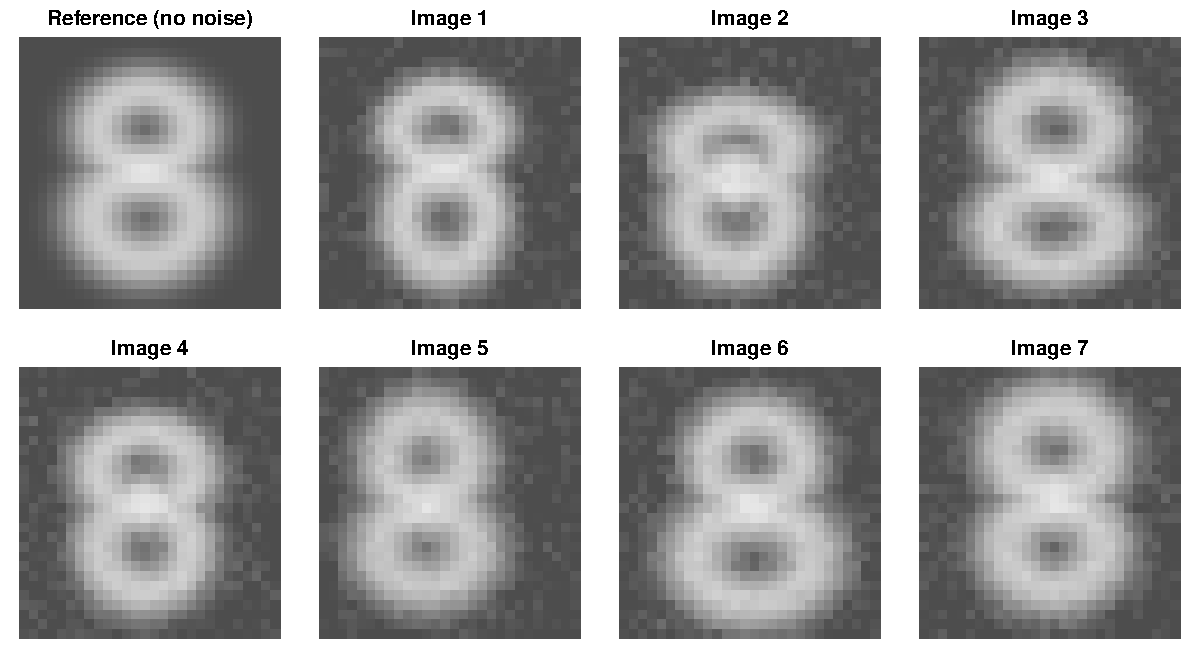
\includegraphics[width=0.85\textwidth]{img/digit-samples.pdf}
  \caption{The noiseless reference digit and seven of the $60$ observed images.}
\end{figure}

\subsubsection{PCA}

We center the data and, since $n = 60 \ll p = 784$, use the small matrix
$\tilde{S} = \frac{1}{n}XX^\top \in \mathbb{R}^{60 \times 60}$:

\begin{lstlisting}
X_centered <- scale(X, center = TRUE, scale = FALSE)
mu <- attr(X_centered, "scaled:center")           # mean image
S_small   <- (1 / n) * X_centered %*% t(X_centered)
eig_small <- eigen(S_small)
lambda  <- eig_small$values;  P_tilde <- eig_small$vectors
head(lambda)
## [1] 2.6141122 1.9787963 1.3592923 0.7745353 0.5222881 0.3148945
keep <- which(lambda > 1e-8)                      # keep the positive eigenvalues
lambda_pos  <- lambda[keep];  P_tilde_pos <- P_tilde[, keep, drop = FALSE]
length(lambda_pos)
## [1] 59
P <- sapply(seq_along(lambda_pos), function(j)
  as.vector(t(X_centered) %*% P_tilde_pos[, j] / sqrt(n * lambda_pos[j])))
dim(P)
## [1] 784  59
\end{lstlisting}

\osservazione{
  \textbf{Why exactly $59$ positive eigenvalues.} The data are centered, so $\operatorname{rank}(\tilde{S}) = \operatorname{rank}(X_c) \leq n - 1 = 59$:
  the constraint $\mathbf{1}_n^\top X_c = 0$ forces at least one zero eigenvalue ($\tilde{S}\mathbf{1}_n = \frac1n X_cX_c^\top\mathbf{1}_n = 0$), and for
  generic data the other $59$ are positive. The tolerance \texttt{1e-8} only discards numerical zeros. Then
  $\bs{p}_j = X^\top\tilde{\bs{p}}_j / \sqrt{n\tilde{\lambda}_j}$ (Suggested exercise 31) gives $59$ orthonormal directions in pixel space
  (numerically $\max|P^\top P - I| \approx 4 \cdot 10^{-14}$).
}

\begin{figure}[H]
  \centering
  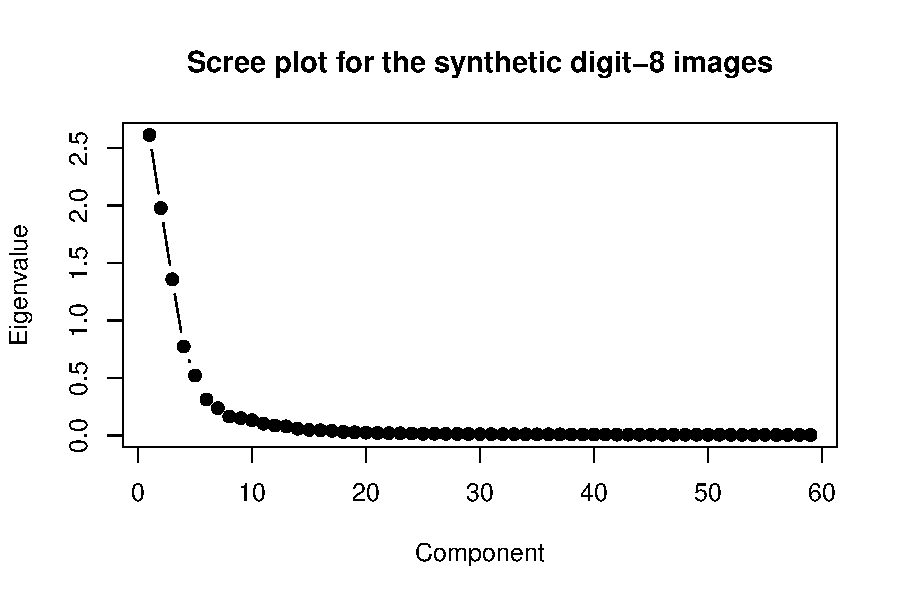
\includegraphics[width=0.6\textwidth]{img/digit-scree.pdf}
  \caption{Scree plot: the first few eigenvalues dominate, because the images vary around a small number of latent shape changes.}
\end{figure}

\subsubsection{Eigenimages}

\dfn{Eigenimage}{
  Each principal direction $\bs{p}_j \in \mathbb{R}^p$ can be reshaped into a $28 \times 28$ array and displayed as an image:
  an \emph{eigenimage}. It is \red{not} an average image: it is a \textbf{direction of variation around the mean image}.
  \begin{itemize}
    \item positive values: pixels that tend to increase together when moving along $\bs{p}_j$;
    \item negative values: pixels that tend to decrease;
    \item large absolute values: pixels most involved in that mode of variation.
  \end{itemize}
}

When the latent score of an image on component $j$ is large and positive, its reconstruction moves from the mean image in
the direction of the eigenimage; when negative, in the opposite direction. For display, a gray scale \textbf{symmetric
around zero} is used (\texttt{zlim = c(-eig\_lim, eig\_lim)}, here \texttt{eig\_lim} $= 0.159$): light and dark are the two signs,
middle gray means small weights.

\begin{figure}[H]
  \centering
  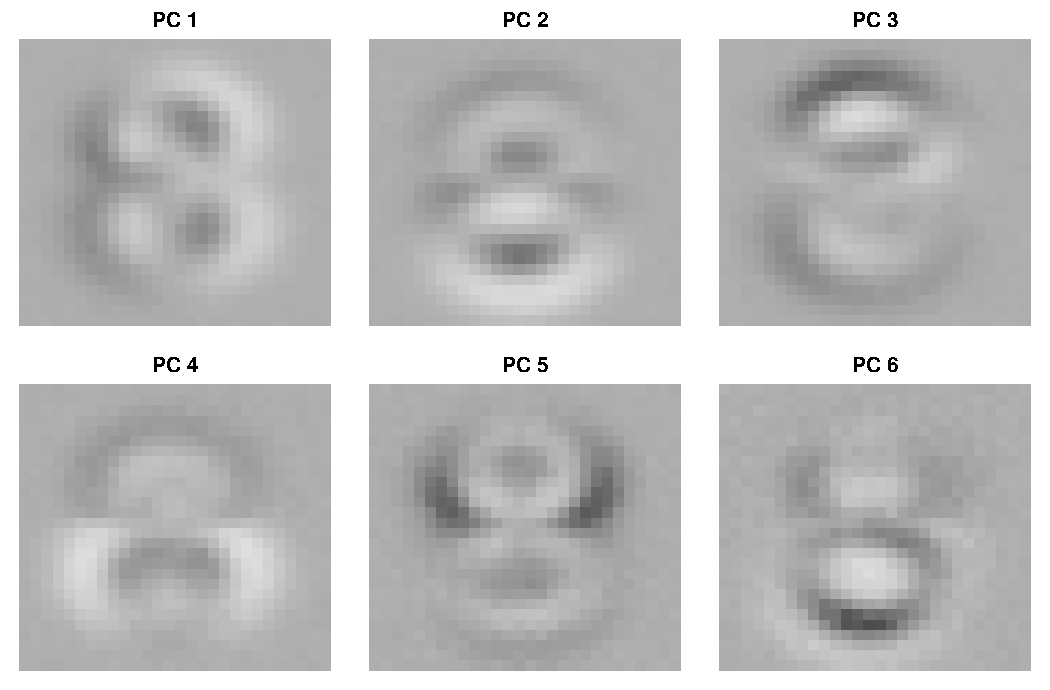
\includegraphics[width=0.75\textwidth]{img/digit-eigenimages.pdf}
  \caption{The first six eigenimages.}
\end{figure}

\subsubsection{Interpretation of the principal directions}

Eigenimages are not easy to read directly. A better way is to look at
\[
  \bar{x} - 2\sqrt{\lambda_j}\,\bs{p}_j, \qquad \bar{x}, \qquad \bar{x} + 2\sqrt{\lambda_j}\,\bs{p}_j ,
\]
because $\lambda_j$ is the variance along the component, so $\sqrt{\lambda_j}$ is its standard deviation: we move by
$\pm 2$ standard deviations from the mean image.

\begin{lstlisting}
mean_img <- matrix(mu, nrow = img_h, ncol = img_w)
pj <- matrix(P[, j], nrow = img_h, ncol = img_w)
minus_img <- mean_img - 2 * sqrt(lambda_pos[j]) * pj
plus_img  <- mean_img + 2 * sqrt(lambda_pos[j]) * pj
# displayed with pmin(pmax(., 0), 1) on the common range [0, 1]
\end{lstlisting}

\begin{figure}[H]
  \centering
  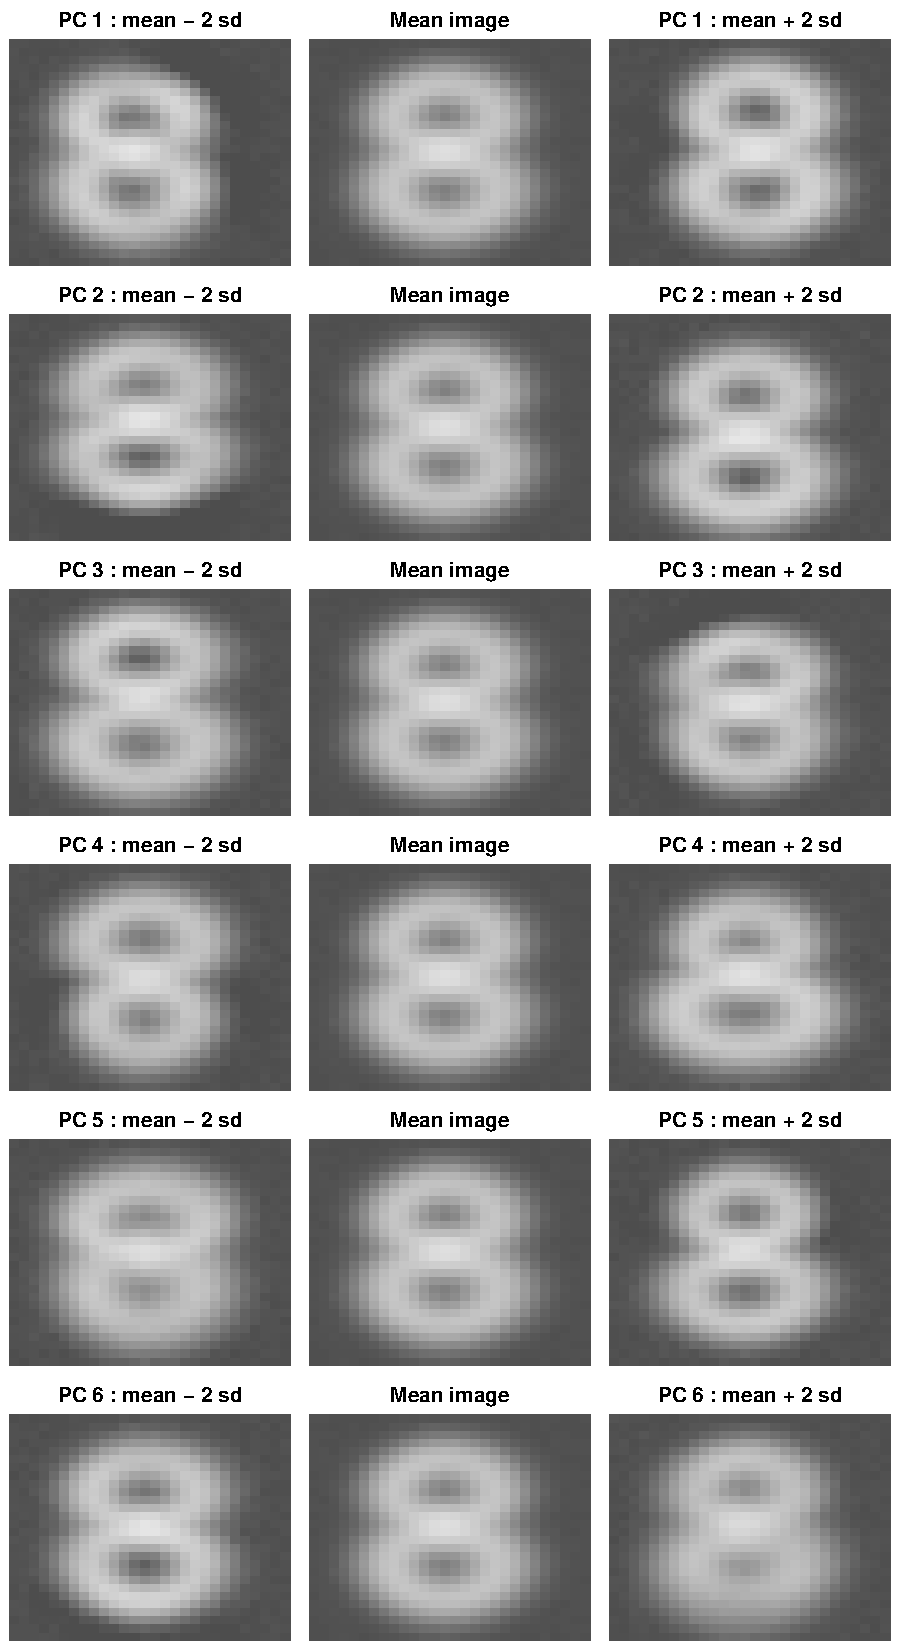
\includegraphics[width=0.55\textwidth]{img/digit-directions.pdf}
  \caption{For each of the first six components: mean $-\,2$ sd, mean image, mean $+\,2$ sd.}
\end{figure}

Some coordinates of the theoretical endpoints lie outside $[0,1]$ and are clipped: the endpoints are points in PCA space
rather than necessarily valid pixel images. With the fixed seed, the first six directions read:
\begin{itemize}
  \item \textbf{PC1 -- horizontal position}: a left--right translation of the whole digit;
  \item \textbf{PC2 -- vertical position}: an up--down displacement, stronger on the lower loop;
  \item \textbf{PC3 -- vertical separation of the loops}: one endpoint brings the loops closer, the other separates them;
  \item \textbf{PC4 -- overall width and stroke thickness}: widening/narrowing of both loops plus apparent thickness;
  \item \textbf{PC5 -- relative loop width}: as one loop becomes wider the other becomes narrower;
  \item \textbf{PC6 -- weaker mixed deformation}: localized changes in loop shape and in the central connection, not tied
        to a single generator parameter.
\end{itemize}

\osservazione{
  The sign of each eigenvector is arbitrary and the order of the later components may change with the simulation.
  These are the dominant shape variations of \emph{this} simulated dataset, not universal features of handwritten 8s.
}

\subsubsection{PCA latent scores}

\begin{lstlisting}
Z <- X_centered %*% P
dim(Z)
## [1] 60 59
head(Z[, 1:3])
##            [,1]       [,2]       [,3]
## [1,] -0.3791712  0.4870712  0.6761959
## [2,] -2.5222515  0.7516631  1.5389542
## [3,]  2.1744691  1.5100075 -0.6520721
## ...
\end{lstlisting}

By the proposition on uncorrelated scores, the columns of $Z$ have mean zero and variances $\lambda_j$ (checked numerically:
the mean of $Z_{\cdot j}^2$ equals $2.614, 1.979, 1.359, \dots$).

\begin{figure}[H]
  \centering
  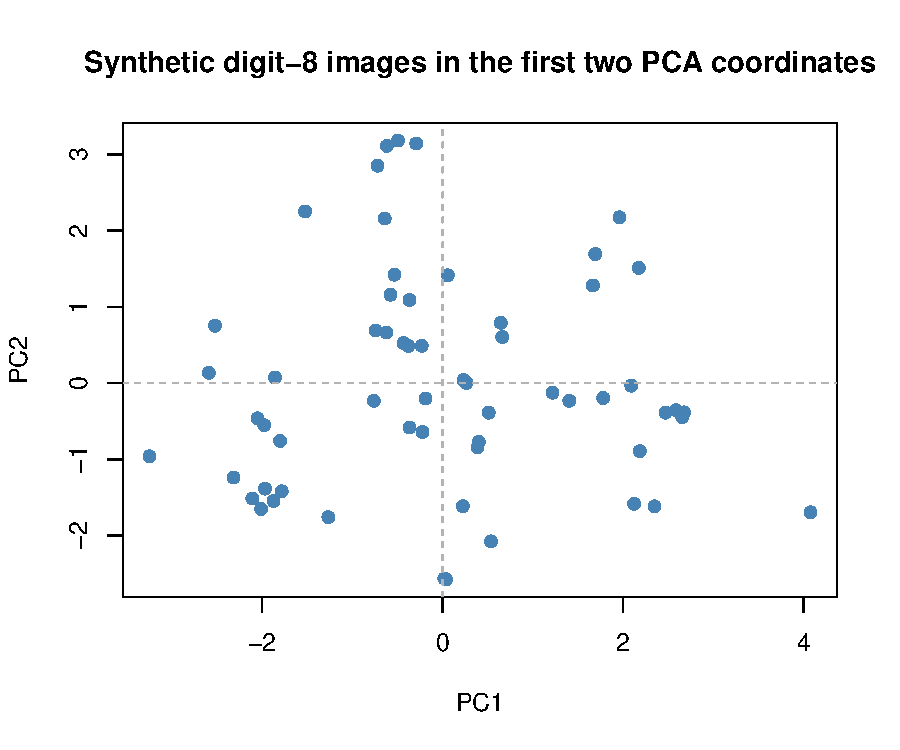
\includegraphics[width=0.6\textwidth]{img/digit-scores.pdf}
  \caption{The $60$ images in the first two PCA coordinates.}
\end{figure}

\osservazione{
  The scatterplot may show denser regions or an apparent grouping. This does \red{not} mean that the images come from
  predefined classes: each image is a combination of a few latent shape variations (horizontal and vertical position,
  relative loop size, thickness, pixel noise), and PCA maps images with similar values of the two dominant ones to nearby
  points. The exact pattern depends on the random seed.
}

\subsubsection{Reconstruction with different numbers of principal components}

\begin{lstlisting}
reconstruct_image <- function(x, P, q, mu) {
  Pq   <- P[, 1:q, drop = FALSE]
  zq   <- (x - mu) %*% Pq                 # scores of the image
  xhat <- zq %*% t(Pq) + mu               # back to pixel space
  matrix(as.vector(xhat), nrow = img_h, ncol = img_w)
}
\end{lstlisting}

i.e.\ $\hat{x} = \bar{x} + P_qP_q^\top(x - \bar{x})$.

\begin{figure}[H]
  \centering
  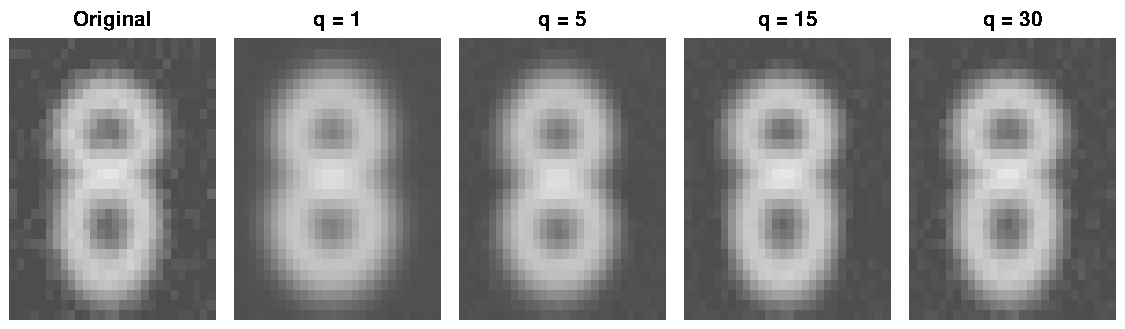
\includegraphics[width=0.95\textwidth]{img/digit-reconstruction.pdf}
  \caption{Image 1 and its reconstructions with $q = 1, 5, 15, 30$ components.}
\end{figure}

\begin{lstlisting}
qs <- c(1, 2, 5, 10, 15, 20, 30, 40)
recon_error <- sapply(qs, function(q) {
  Pq <- P[, 1:q, drop = FALSE]
  Xhat <- X_centered %*% Pq %*% t(Pq)
  mean(rowSums((X_centered - Xhat)^2))
})
\end{lstlisting}

\begin{center}
\begin{tabular}{c|cccccccc}
  $q$ & 1 & 2 & 5 & 10 & 15 & 20 & 30 & 40 \\
  \hline
  error & 6.629 & 4.650 & 1.994 & 0.988 & 0.607 & 0.430 & 0.256 & 0.144
\end{tabular}
\end{center}

\begin{figure}[H]
  \centering
  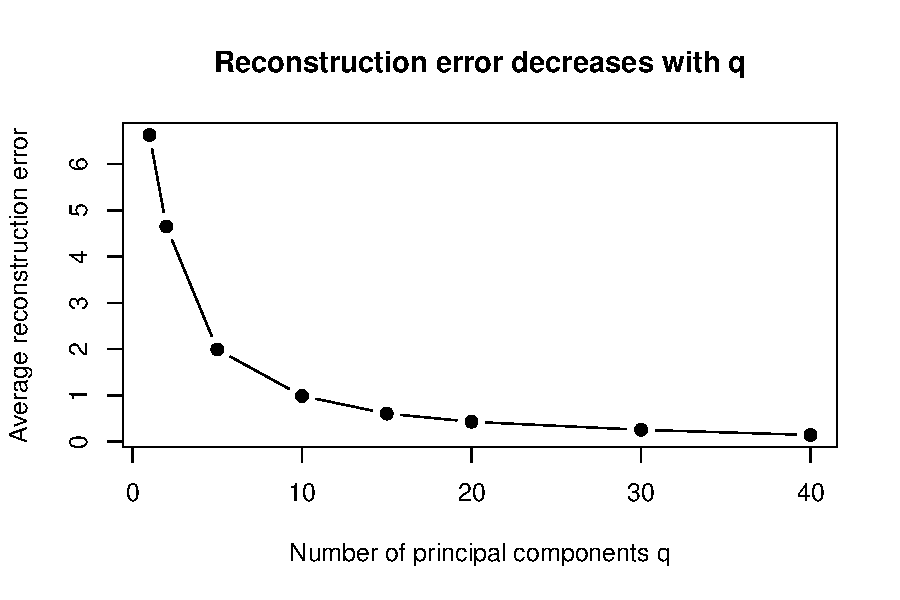
\includegraphics[width=0.6\textwidth]{img/digit-recon-error.pdf}
  \caption{The average reconstruction error decreases with $q$.}
\end{figure}

\esempio{
  \begin{itemize}
    \item The table is the theory in numbers: the error for $q$ components equals exactly the lost variance
          $J = \sum_{j > q}\lambda_j$ (checked in R to all printed digits), and it reaches $0$ at $q = 59$.
    \item The total variance is $J_0 = \sum_j\lambda_j \approx 6.63 + 2.61 = 9.24$, so $q = 5$ already keeps about $78\%$ of it and $q = 15$ about $93\%$:
          with $15$ numbers instead of $784$ the digit is visually almost identical to the original.
    \item Eckart--Young check: with the SVD of the centered data and $q = 5$, \texttt{norm(X\_centered - Xq, "2")} and
          $\sigma_6$ both equal $4.346685$; and $\sigma_j^2/n = \lambda_j$ up to $10^{-14}$.
  \end{itemize}
}
